\documentclass[compress]{beamer}
\usepackage{ifthen,verbatim}

\title{Overlap-hits under the microscope}
\author{Jim Pivarski, Alexei Safonov, K\'aroly Banicz$^*$}
\institute{Texas A\&M University, $^*$US-CMS}
\date{14 July, 2008}

\newcommand{\isnote}{}
\xdefinecolor{lightyellow}{rgb}{1.,1.,0.25}
\xdefinecolor{darkblue}{rgb}{0.1,0.1,0.7}

%% Uncomment this to get annotations
%% \def\notes{\addtocounter{page}{-1}
%%            \renewcommand{\isnote}{*}
%% 	   \beamertemplateshadingbackground{lightyellow}{white}
%%            \begin{frame}
%%            \frametitle{Notes for the previous page (page \insertpagenumber)}
%%            \itemize}
%% \def\endnotes{\enditemize
%% 	      \end{frame}
%%               \beamertemplateshadingbackground{white}{white}
%%               \renewcommand{\isnote}{}}

%% Uncomment this to not get annotations
\def\notes{\comment}
\def\endnotes{\endcomment}

\setbeamertemplate{navigation symbols}{}
\setbeamertemplate{headline}{\mbox{ } \hfill
\begin{minipage}{5.5 cm}
\vspace{-0.75 cm} \small
\end{minipage} \hfill
\begin{minipage}{4.5 cm}
\vspace{-0.75 cm} \small
\begin{flushright}
\ifthenelse{\equal{\insertpagenumber}{1}}{}{Jim Pivarski \hspace{0.2 cm} \insertpagenumber\isnote/\pageref{numpages}}
\end{flushright}
\end{minipage}\mbox{\hspace{0.2 cm}}\includegraphics[height=1 cm]{../cmslogo} \hspace{0.1 cm} \includegraphics[height=1 cm]{../tamulogo} \hspace{0.01 cm} \vspace{-1.05 cm}}

\begin{document}
\frame{\titlepage}

%% \begin{notes}
%% \item This is the annotated version of my talk.
%% \item If you want the version that I am presenting, download the one
%% labeled ``slides'' on Indico (or just ignore these yellow pages).
%% \item The annotated version is provided for extra detail and a written
%% record of comments that I intend to make orally.
%% \item Yellow notes refer to the content on the {\it previous} page.
%% \item All other slides are identical for the two versions.
%% \end{notes}

\begin{frame}
\frametitle{Rationale}
\begin{itemize}\setlength{\itemsep}{0.2 cm}
\item HIPAlignmentAlgorithm properly treats the correlation between $x$ and
$y$, assuming that these are both continuous random variables with
Gaussian errors.

\item Both $x$ and $y$ distributions have structure: narrow Gaussian
  peak when the muon passes between strips/wire groups, flat
  distribution when the muon passes through strips/wire groups.

\item Separation between $y$ wire groups is much greater than our
  desired alignment precision (1.5~cm in ME+2/1, 5~cm in ME+2/2), so
  granularity in $y$ could cause serious artifacts.

\item These propagate into $x$ because the strips are angled.

\end{itemize}

\vspace{0.2 cm}
\hspace{-0.83 cm} \textcolor{darkblue}{\Large Exploratory study}

\vspace{0.15 cm}
\begin{itemize}
\item Made an ntuple of hit positions and residuals; looked at what we're starting with
\end{itemize}

\end{frame}

\begin{frame}
\frametitle{Distribution of hits}
\scriptsize
\begin{itemize}
\item Edge of trapezoid is clearly visible
\item As are the wire groups in $y$
\item I don't understand the gap on the far left edge or the small half-integer peaks
\item This isn't discovery: CSCRecHits are constructed to have this distribution
\item ME+2/2 has 5~cm between wire group centers
\end{itemize}

\vfill
\begin{columns}
\column{0.5\linewidth}
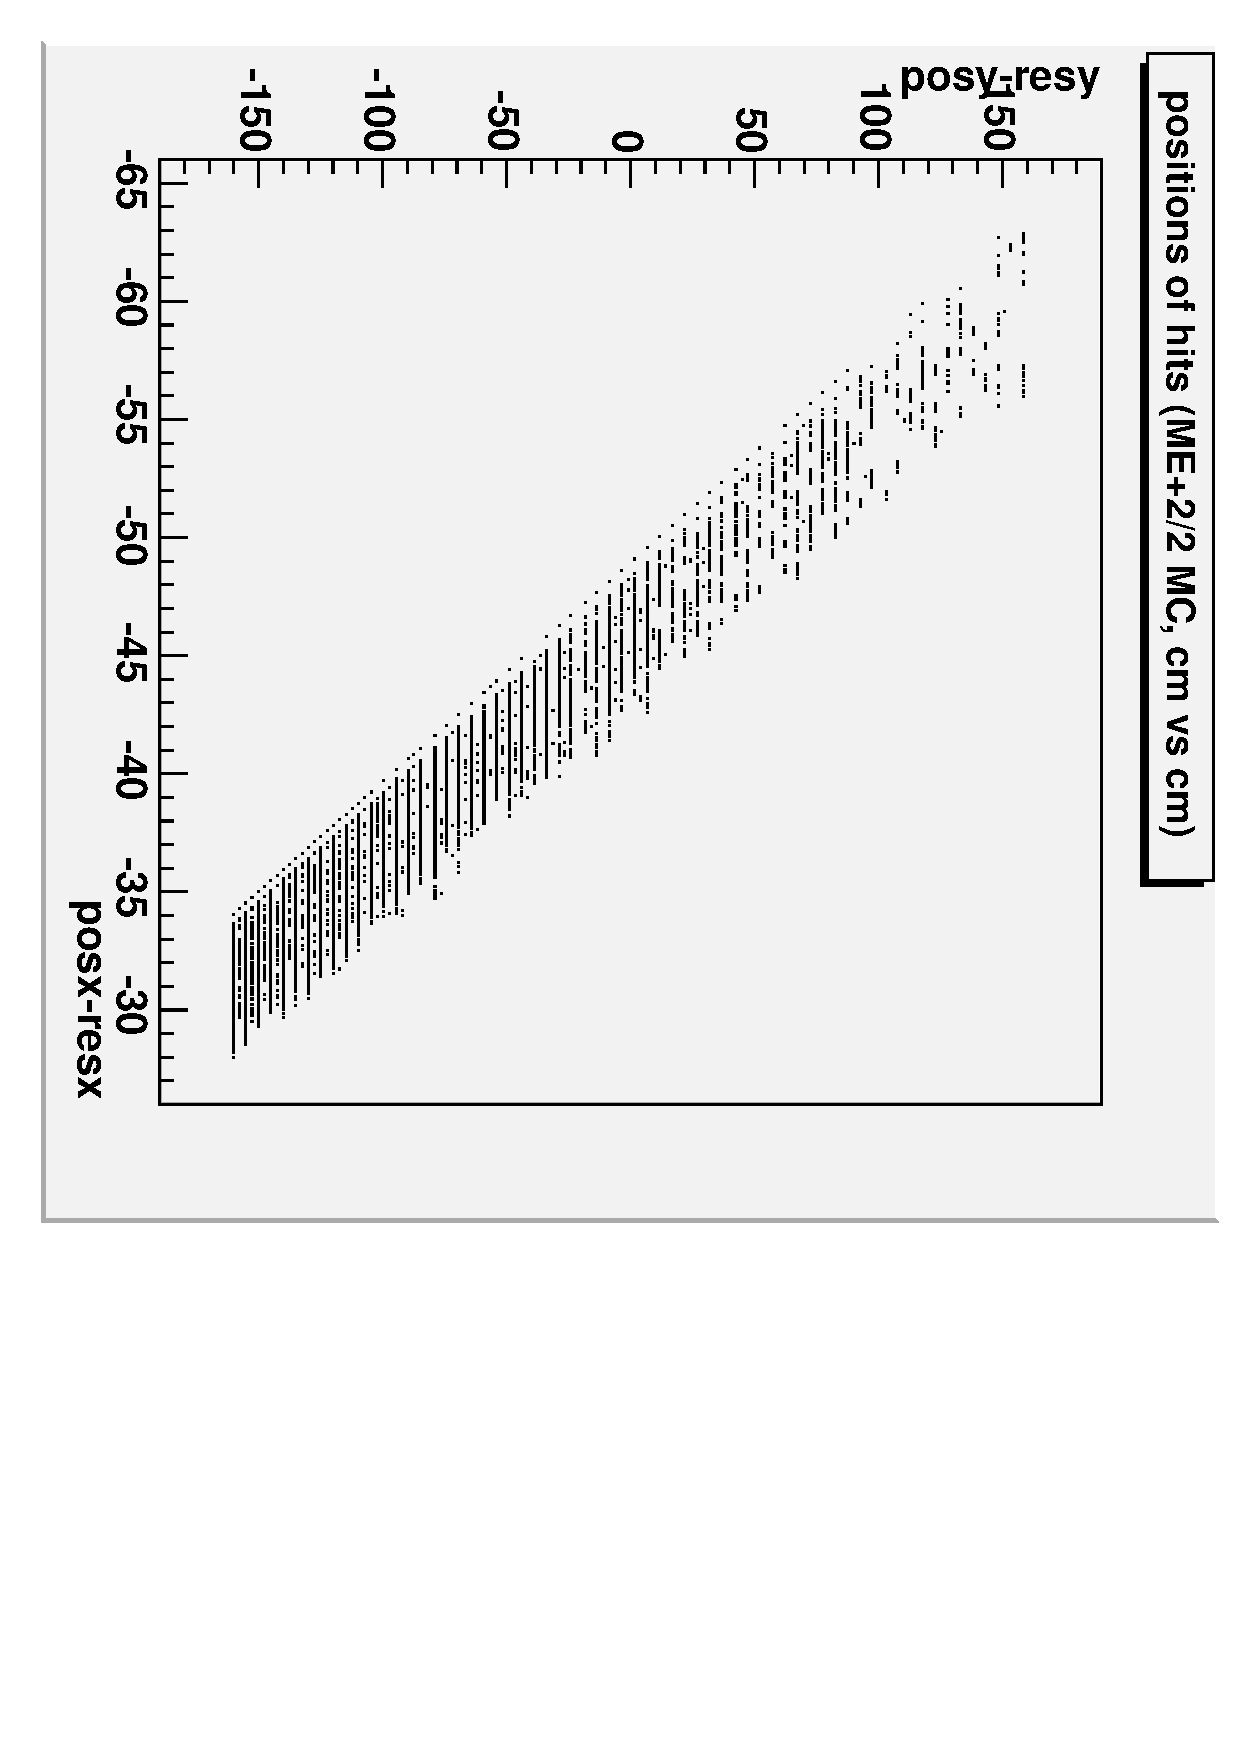
\includegraphics[height=\linewidth, angle=90]{MC_positions_of_hits.pdf}
\column{0.5\linewidth}
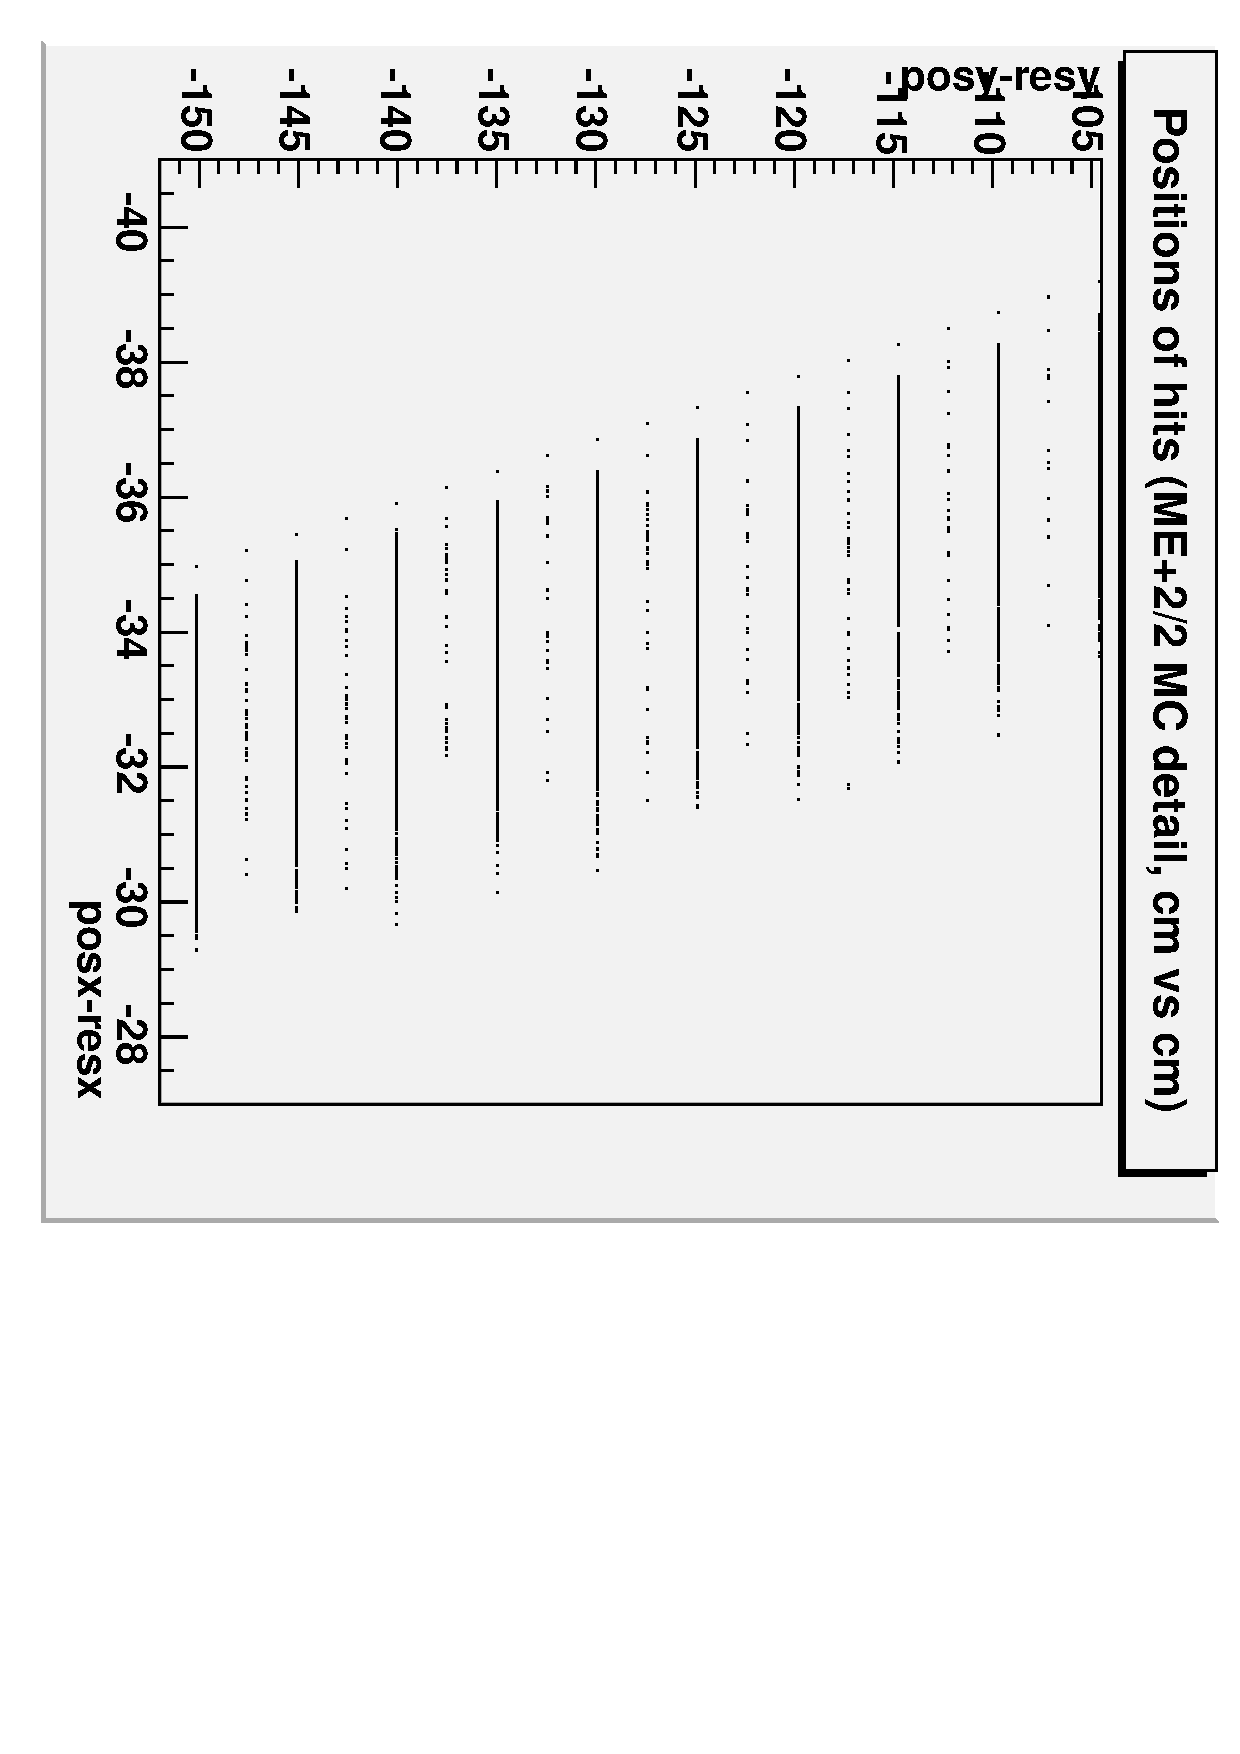
\includegraphics[height=\linewidth, angle=90]{MC_positions_of_hits_detail.pdf}
\end{columns}
\end{frame}

\begin{frame}
\frametitle{Distribution of impact points}
\scriptsize
\begin{itemize}
\item Propagate tracks from reference chamber, plot them in local coordinates of target chamber
\item Clearly see the angle between the two chambers
\item Some broadening because tracks are not perfectly parallel
\item In {\it cosmics} data, complete smearing because tracks are nowhere near parallel
\end{itemize}

\vfill
\begin{columns}
\column{0.5\linewidth}
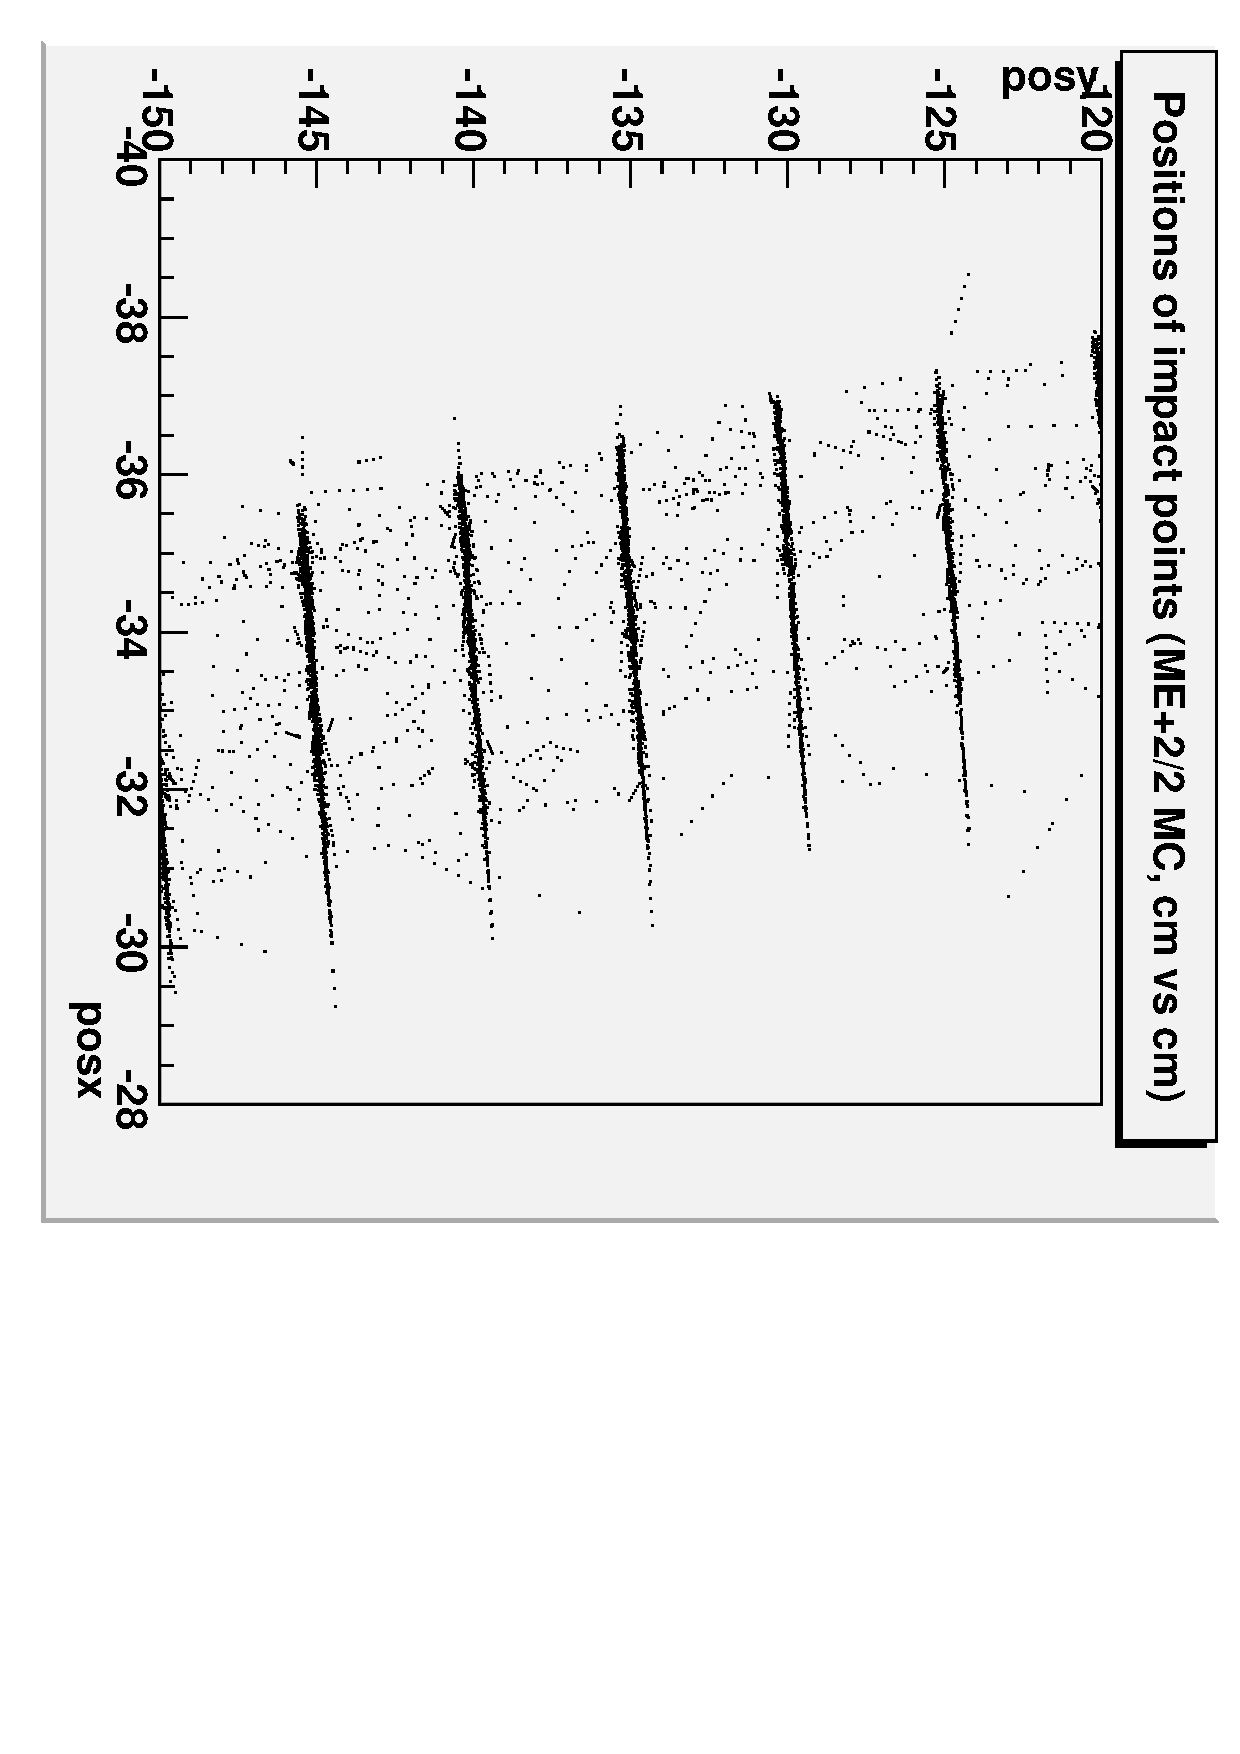
\includegraphics[height=\linewidth, angle=90]{MC_positions_of_impact_points_detail.pdf}
\column{0.5\linewidth}
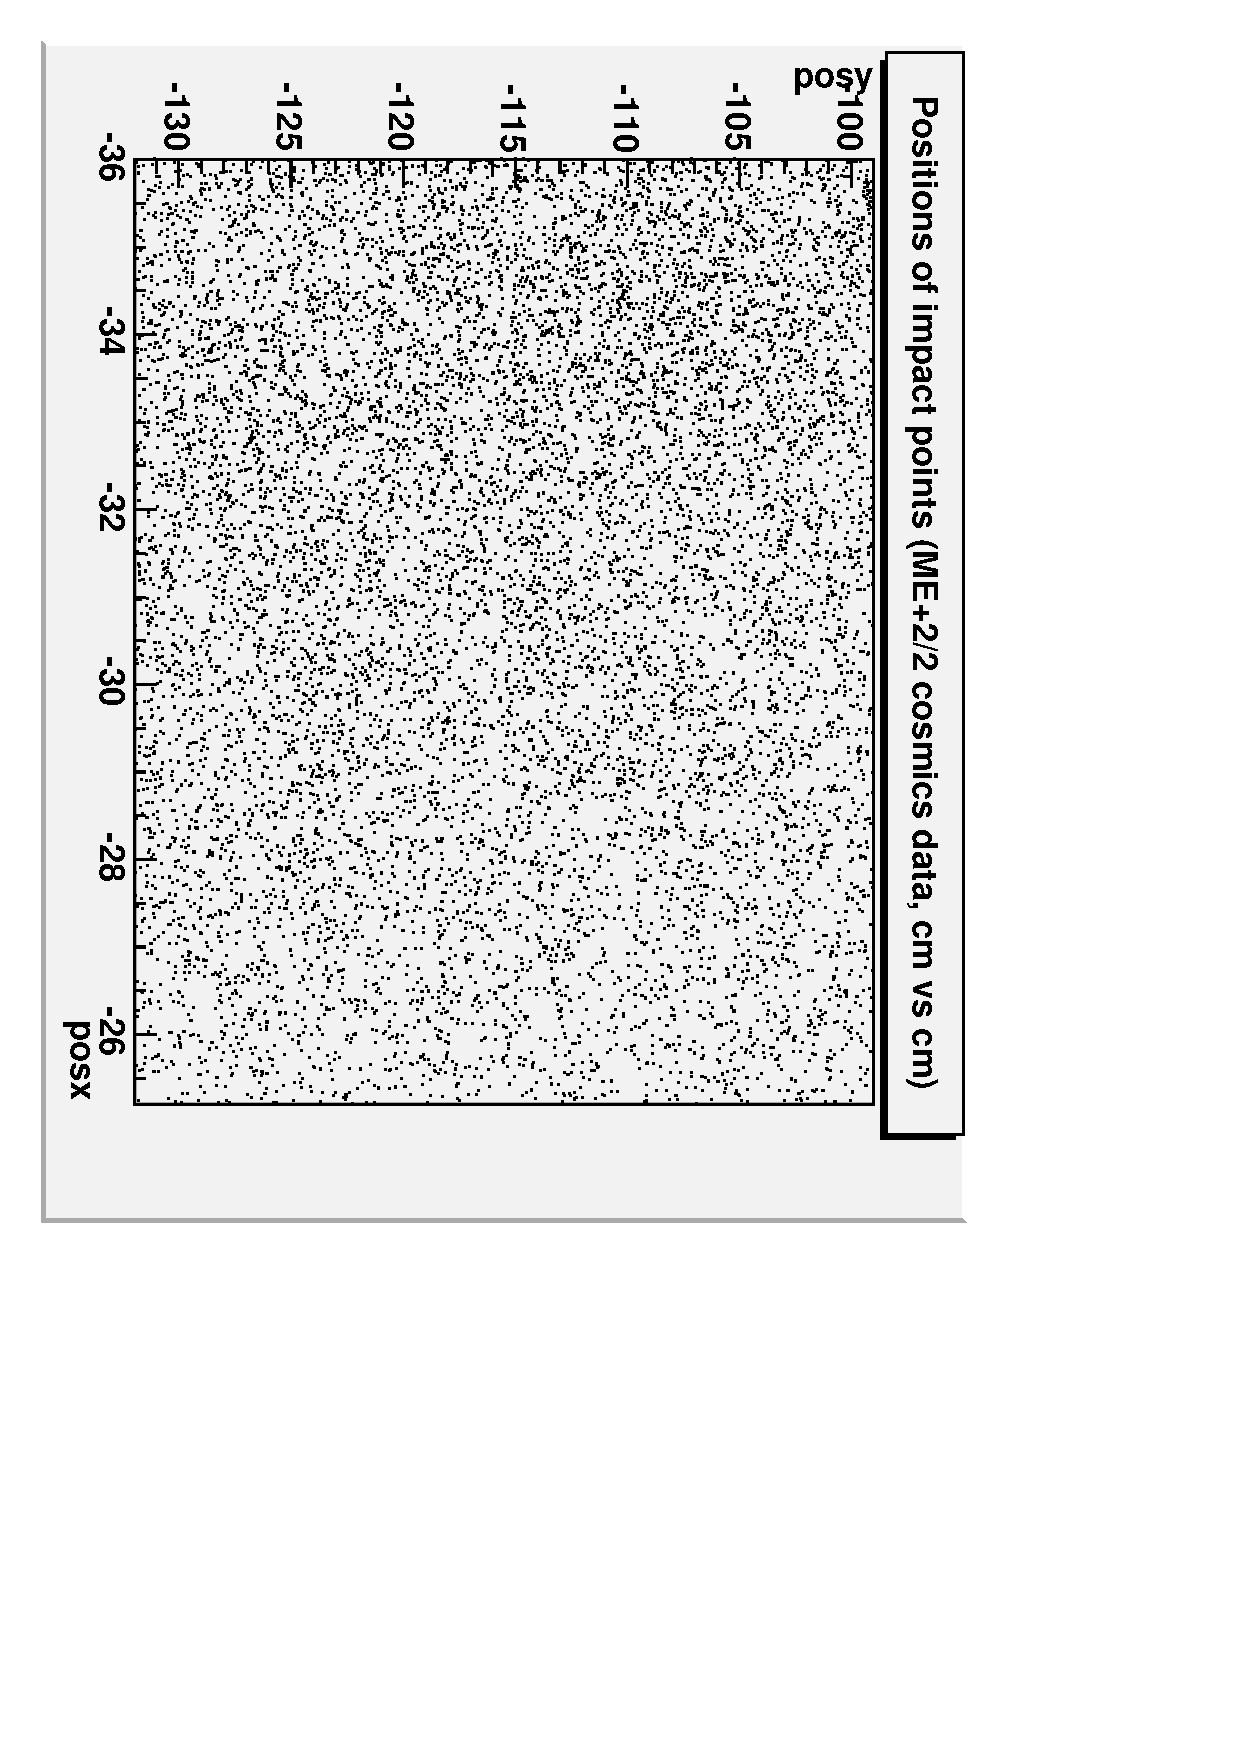
\includegraphics[height=\linewidth, angle=90]{data_impact-points_ME22.pdf}
\end{columns}
\end{frame}

\begin{frame}
\frametitle{Residuals}
\scriptsize
\begin{itemize}
\item 2-D residual distribution: expect
\begin{itemize}
\item \scriptsize correlation between $x$ and $y$ because $x$ can only be determined from strip if $y$ is known
\item \scriptsize peaks in $y$ corresponding to $\pm$0, $\pm$1,
  $\pm$2\ldots\ differences in wire groups from reference to target
\end{itemize}
\item Observed both features: slope is 0.1, central peak has vast majority of the events
\item Inner $|r_y|$ $<$ 2~mm is featureless
\end{itemize}

\vfill
\begin{columns}
\column{0.5\linewidth}
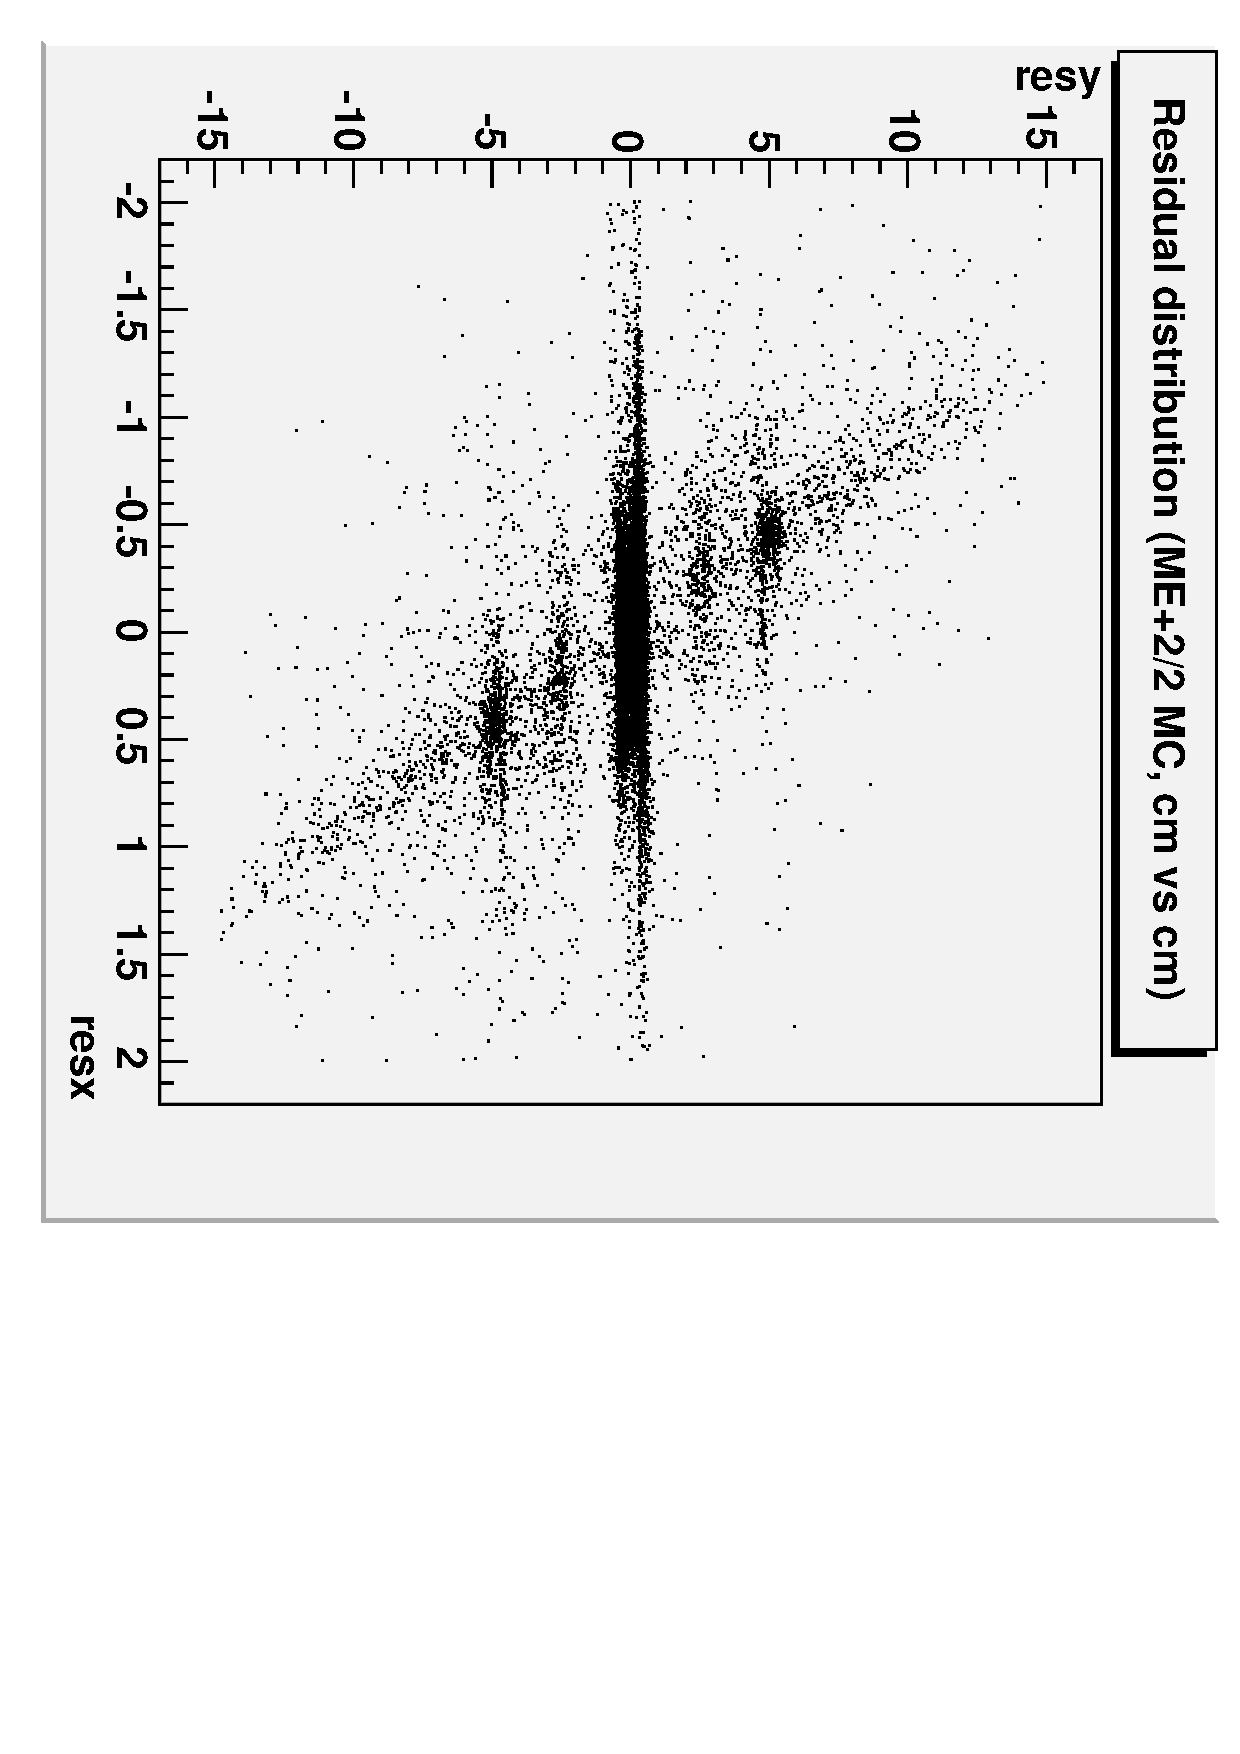
\includegraphics[height=\linewidth, angle=90]{MC_residuals.pdf}
\column{0.5\linewidth}
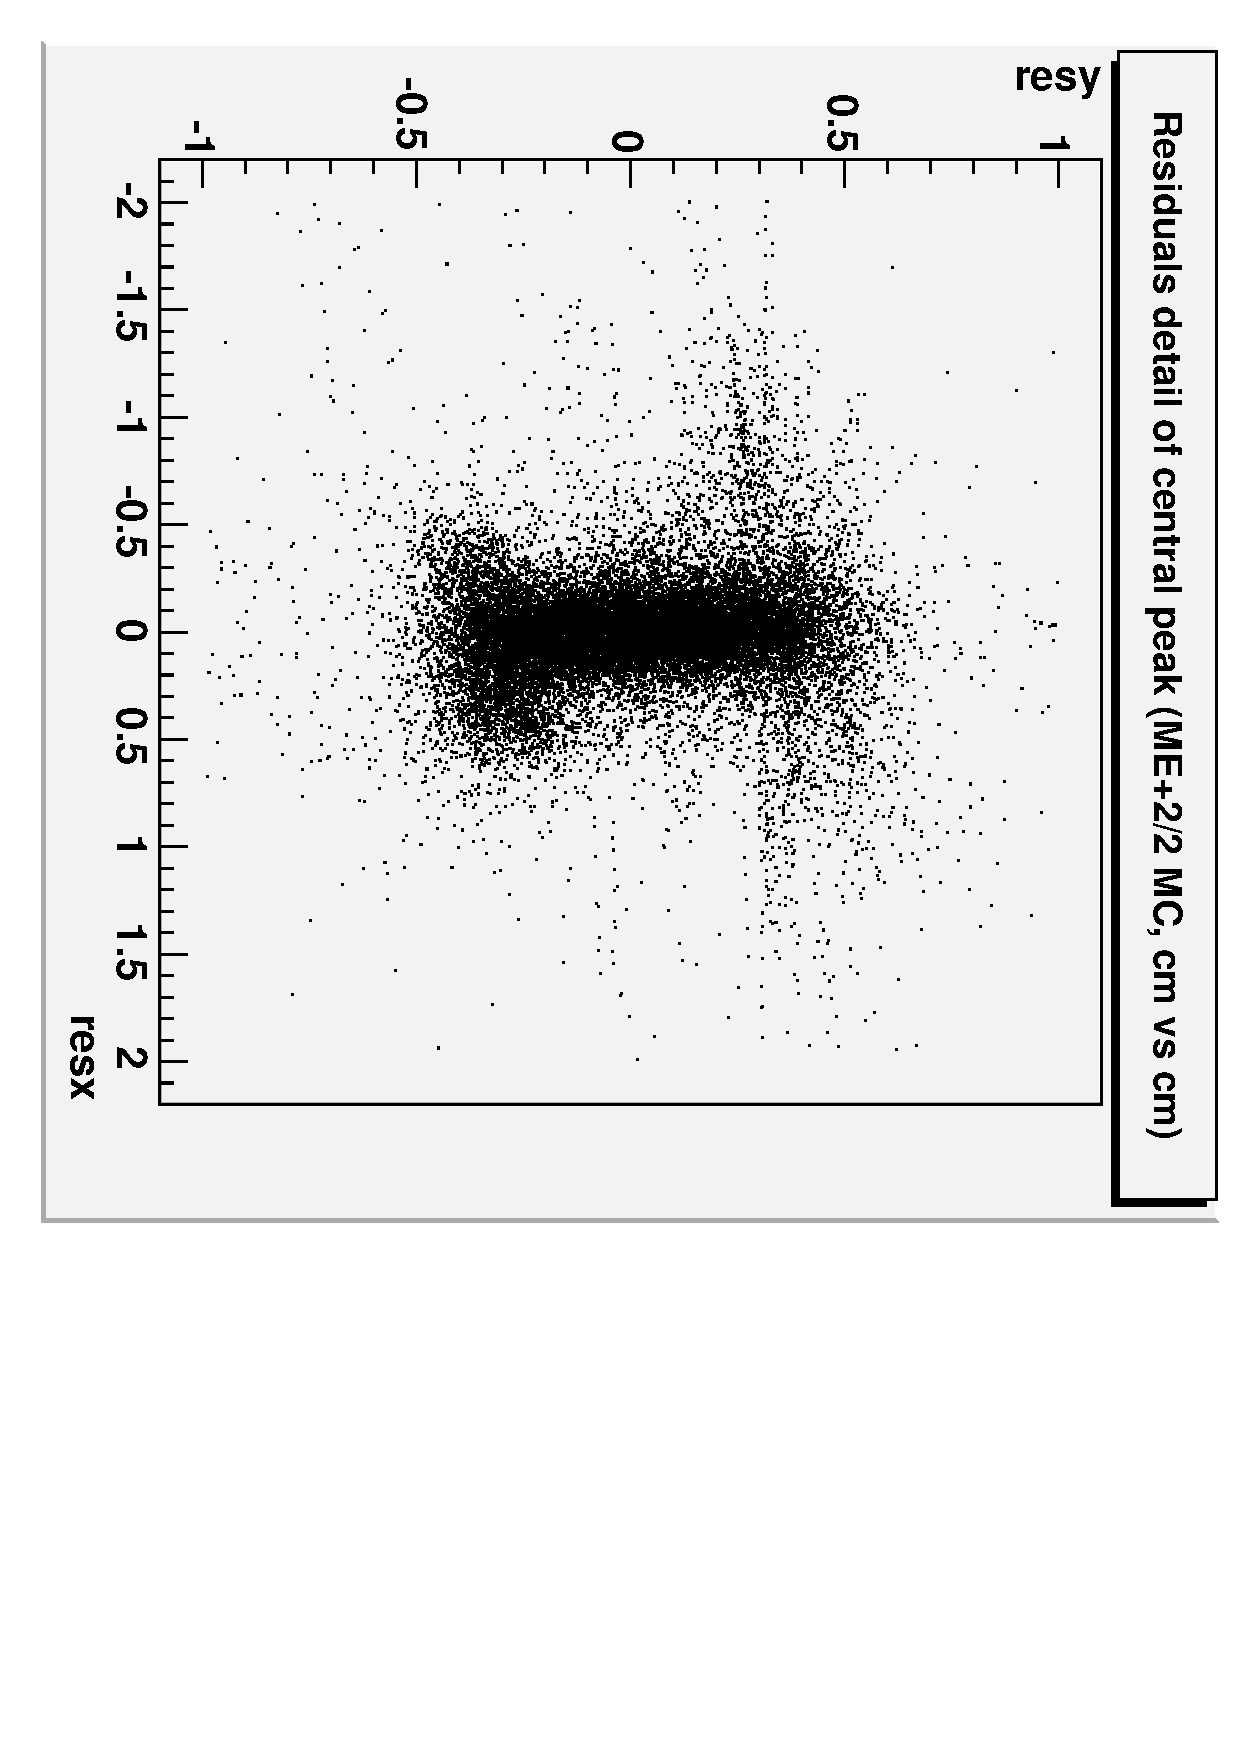
\includegraphics[height=\linewidth, angle=90]{MC_residuals_detail.pdf}
\end{columns}
\end{frame}

\begin{frame}
\frametitle{Residuals in data}
\scriptsize
\begin{itemize}
\item Look at the same distributions in CRUZET data
\item Same correlation, but structure is entirely washed out
\item More to do with the fact that these are cosmics than the fact that these are data
\item (Yes, we only look at one chamber at a time in data.  This one has the most hits.)
\end{itemize}

\vfill
\begin{columns}
\column{0.5\linewidth}
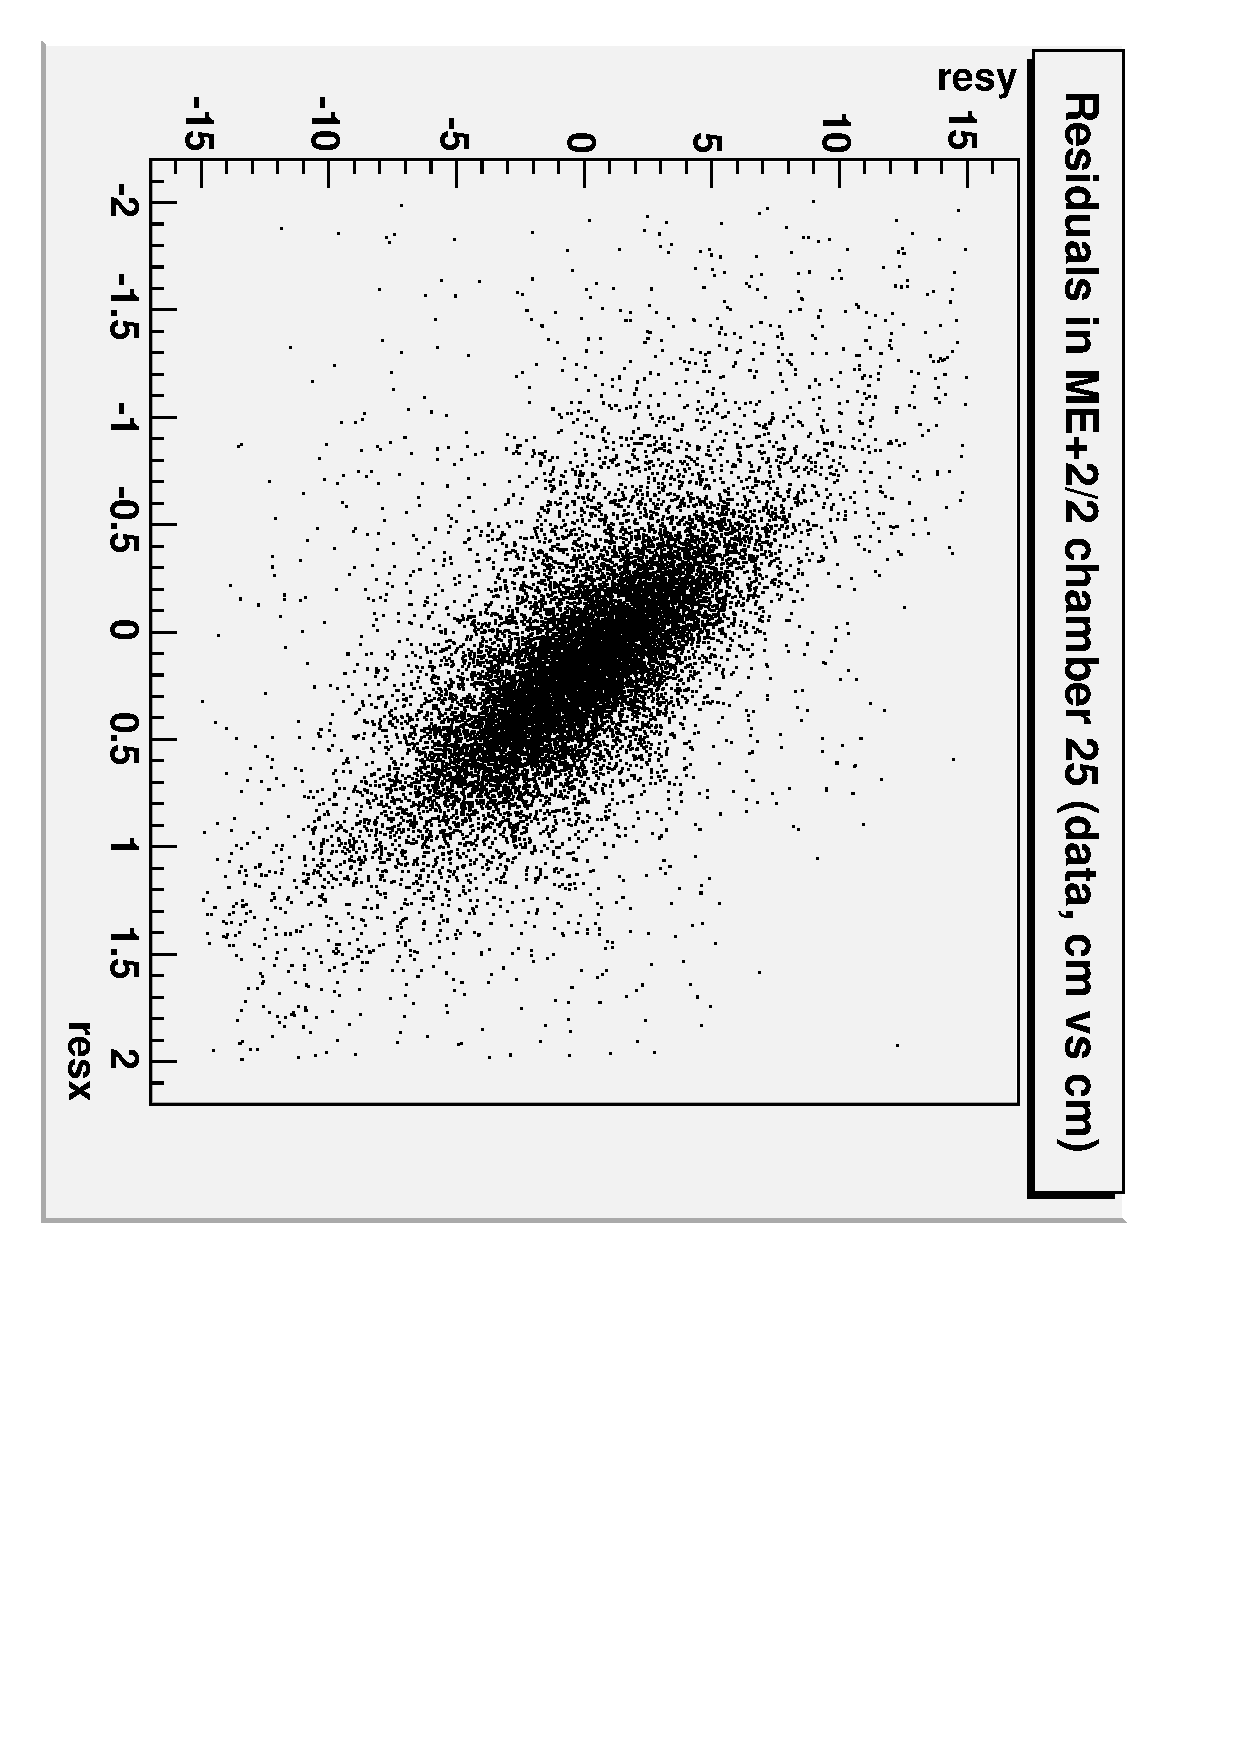
\includegraphics[height=\linewidth, angle=90]{data_residuals_ME22.pdf}
\column{0.5\linewidth}
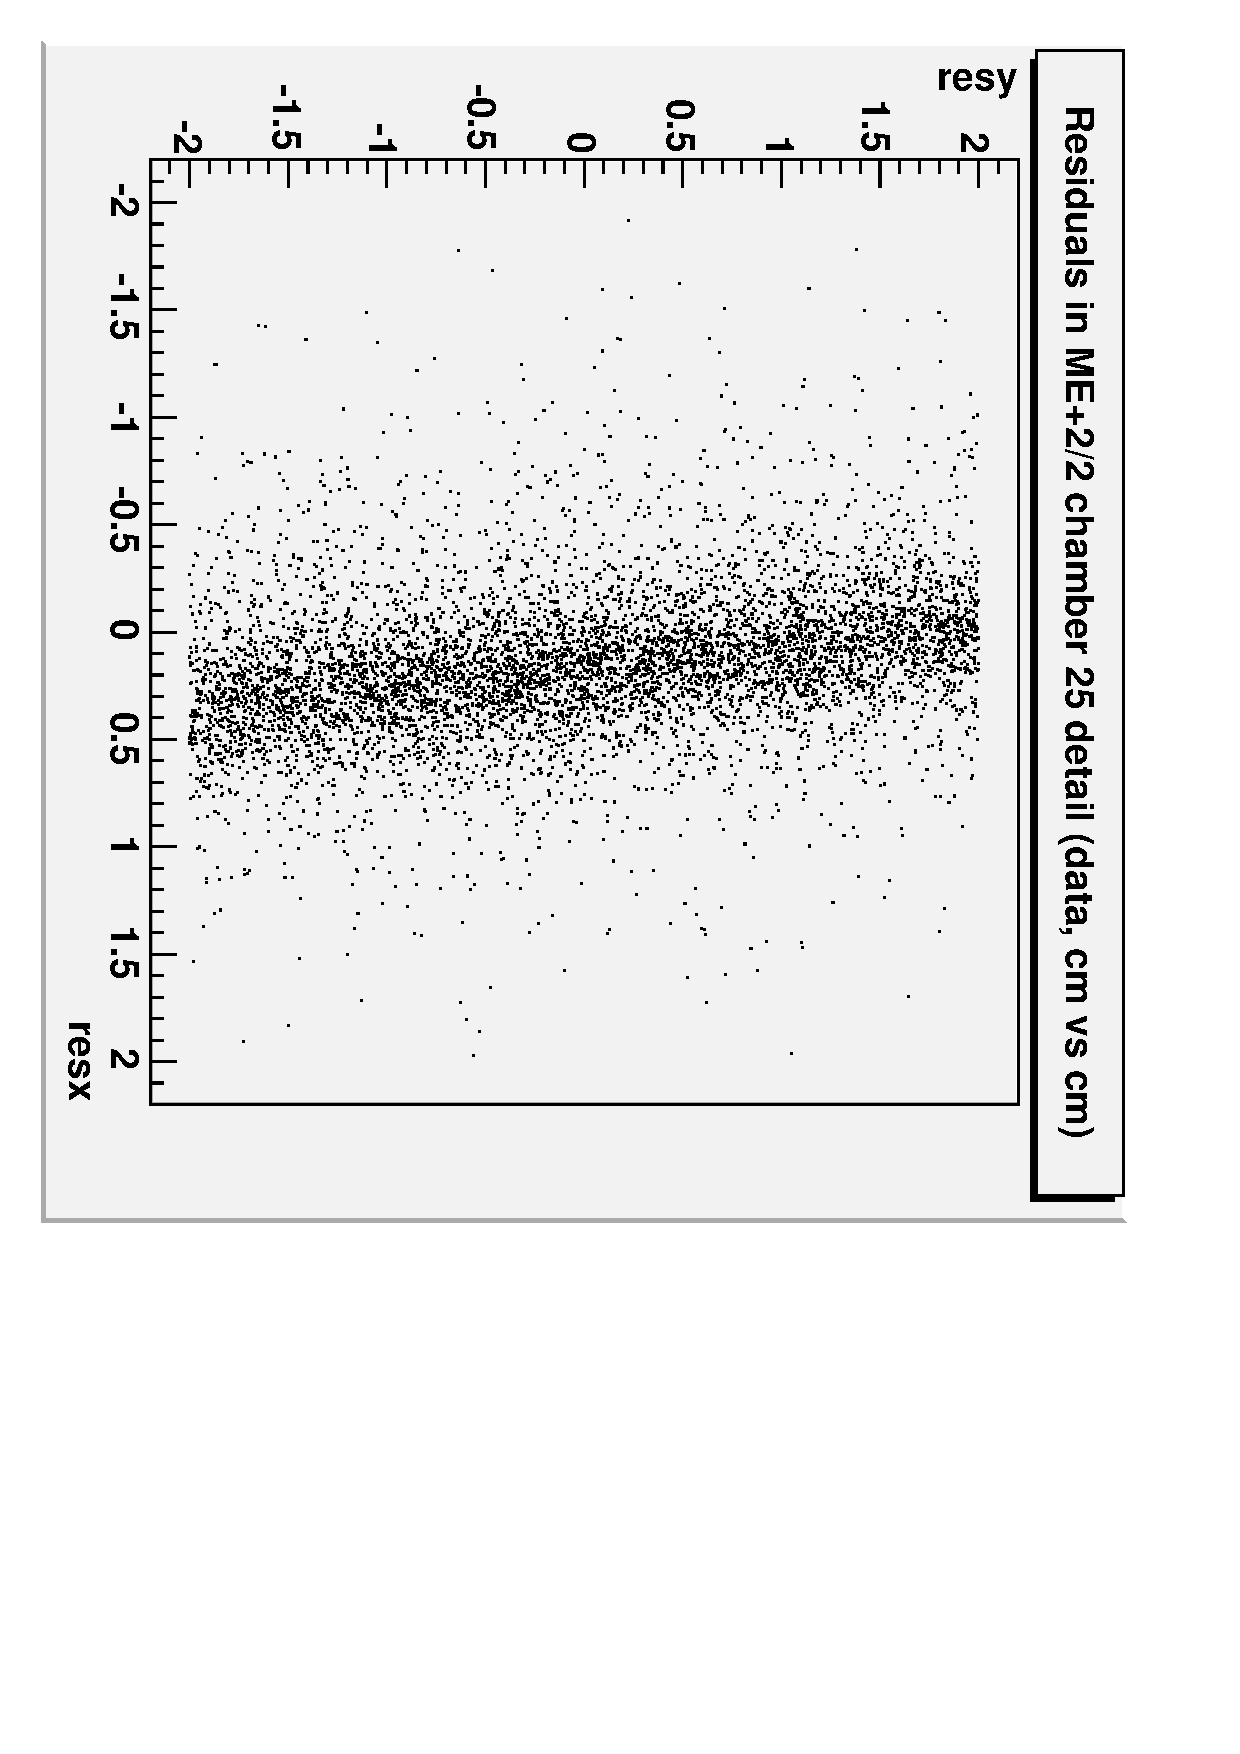
\includegraphics[height=\linewidth, angle=90]{data_residuals_ME22_detail.pdf}
\end{columns}
\end{frame}

\begin{frame}
\frametitle{Why are cosmics smeared?}

\vfill
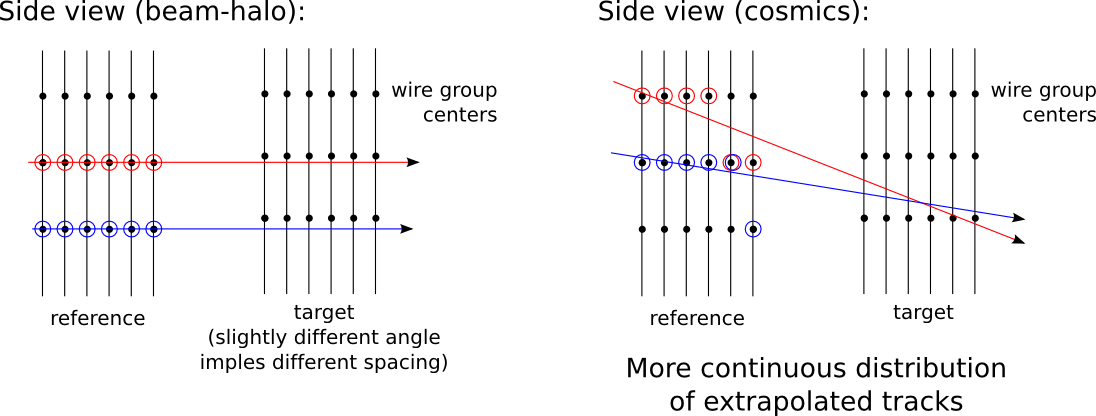
\includegraphics[width=\linewidth]{why_cosmics_smeared.png}

\begin{columns}
\column{0.4\linewidth}
\scriptsize

Quantify angles of tracks with local $\partial y/\partial z$

\vspace{0.1 cm}
Close to zero in beam-halo MC

\vspace{0.1 cm} Clear shape in cosmic ray data
\begin{itemize}
\item cosmic rays steeply angled relative to beamline

\item preference for negative $\partial y/\partial z$, points to interaction point (ALCT patterns)

\item slope of 1 means a new wire group every two layers

\end{itemize}

\column{0.6\linewidth}
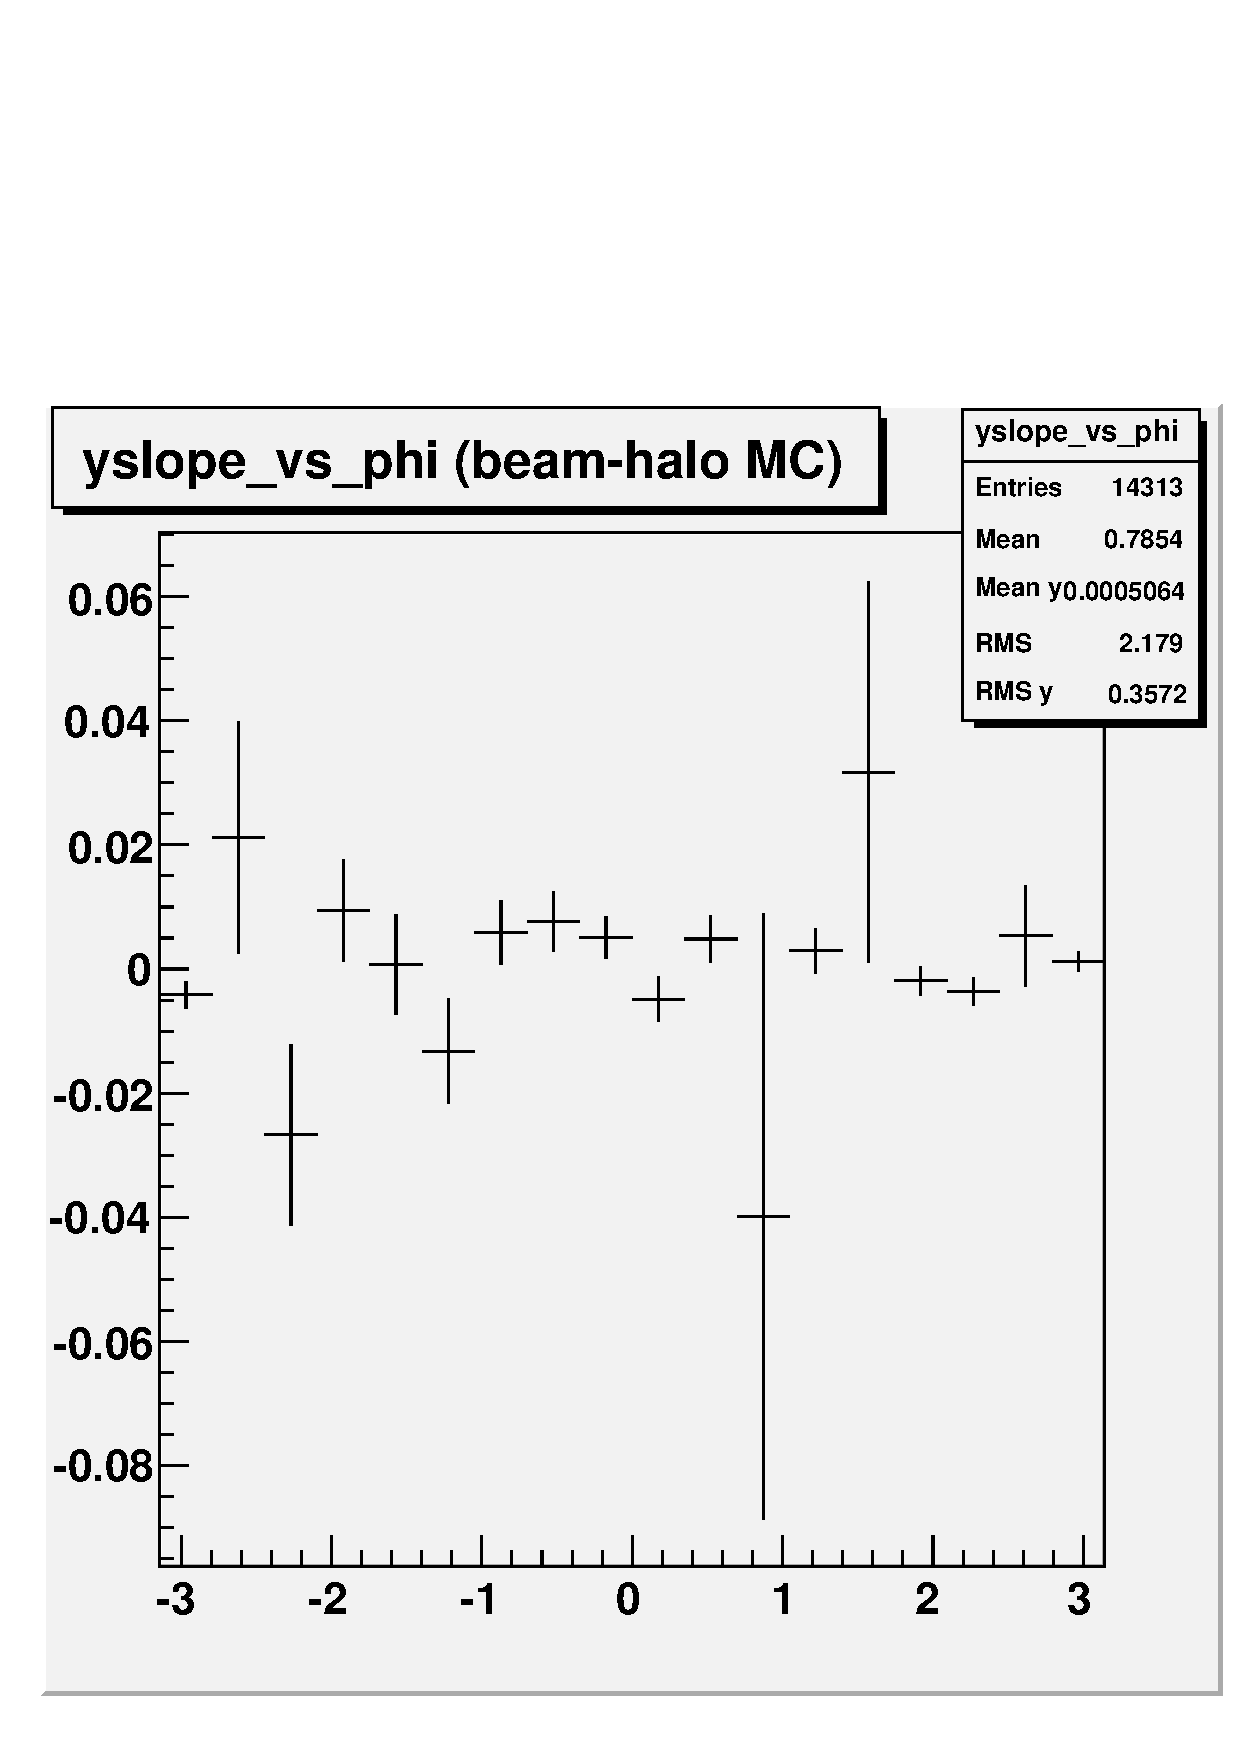
\includegraphics[width=0.5\linewidth]{MC_yslope_vs_phi.pdf}
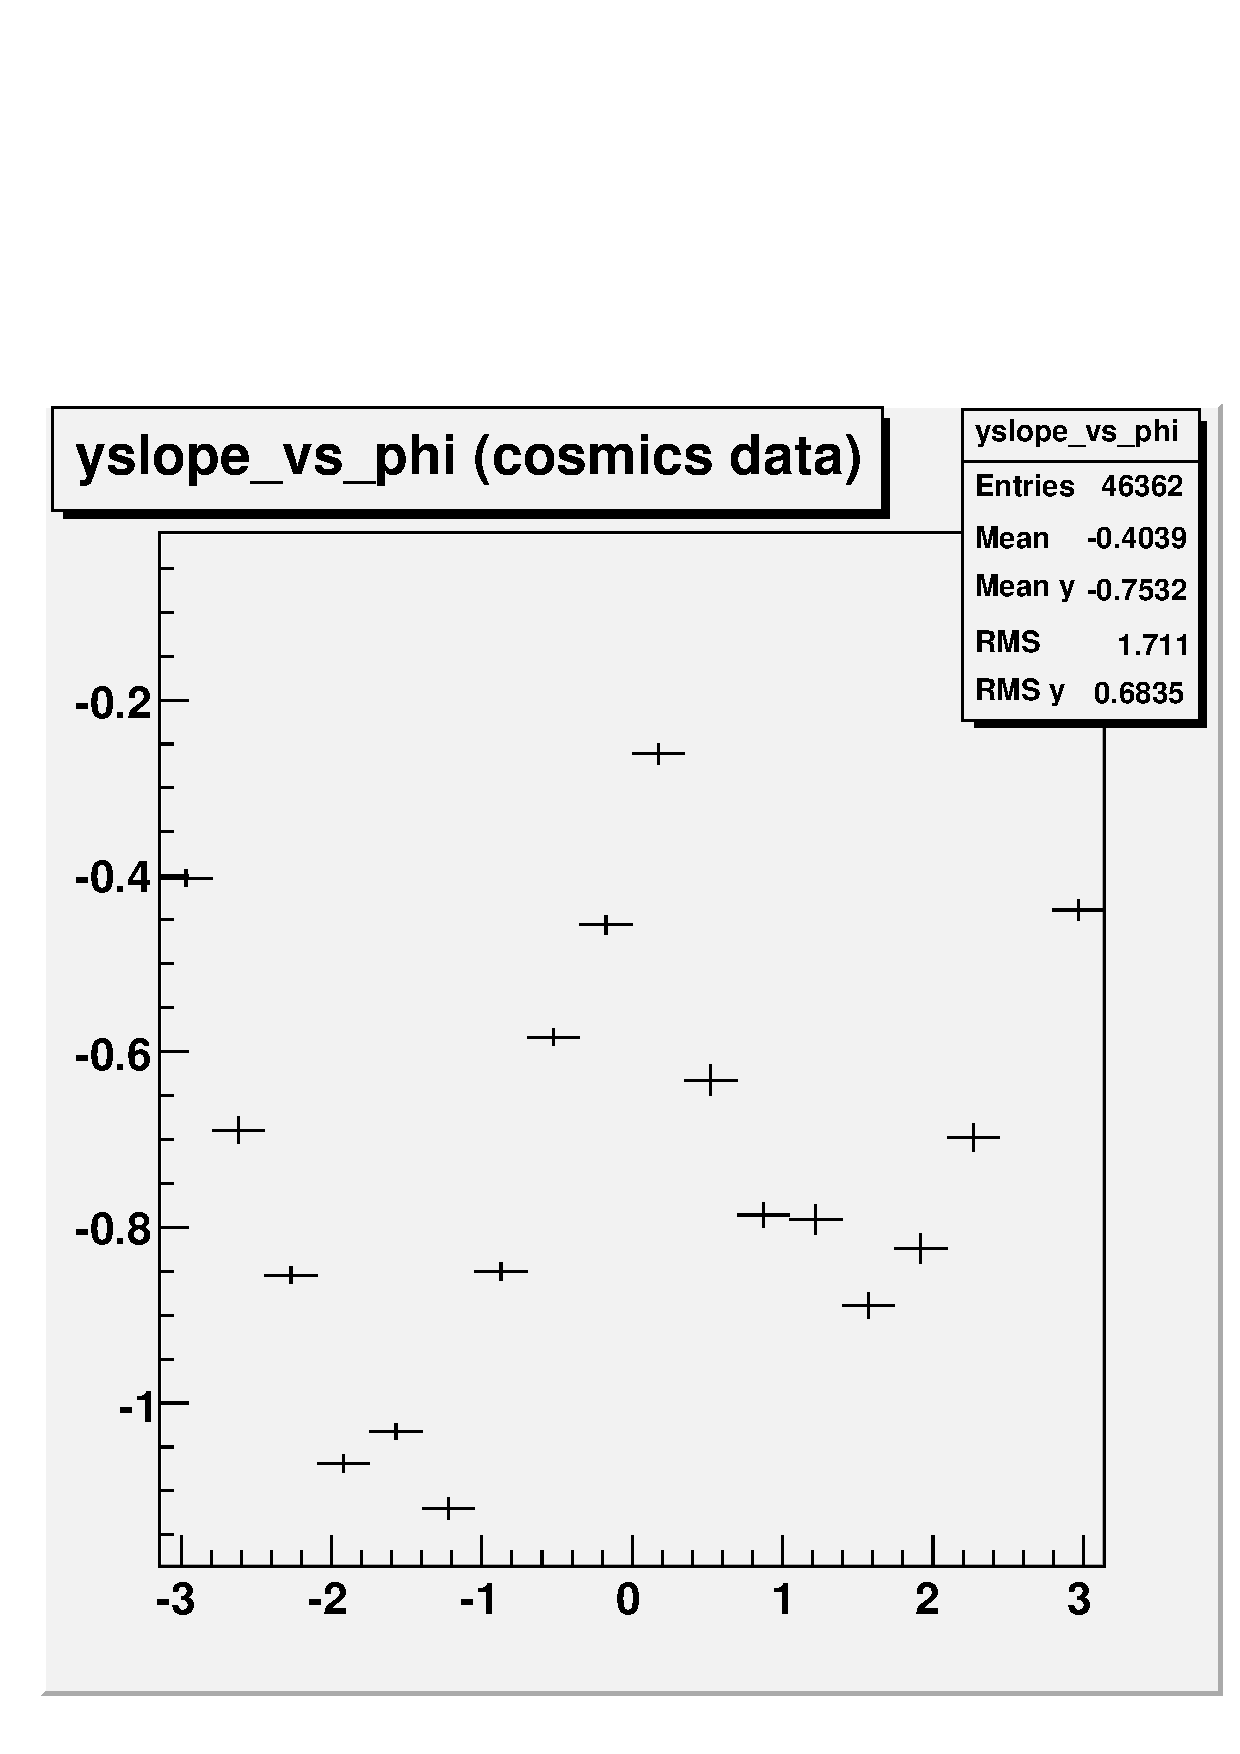
\includegraphics[width=0.5\linewidth]{data_yslope_vs_phi.pdf}
\end{columns}
\end{frame}

\begin{frame}
\frametitle{Granularity in beam-halo (1/2)}
\scriptsize
\begin{itemize}
\item Can deal with granularity in the beam-halo ME+2/2 case (biggest separation between peaks) by selecting events in good region of the $\Delta y$ = 0 peak
\item In this region, we have a flat probability distribution in $y$
\item (Not as important right now as the cosmic-ray case)
\end{itemize}

\vfill
\begin{columns}
\column{0.5\linewidth}
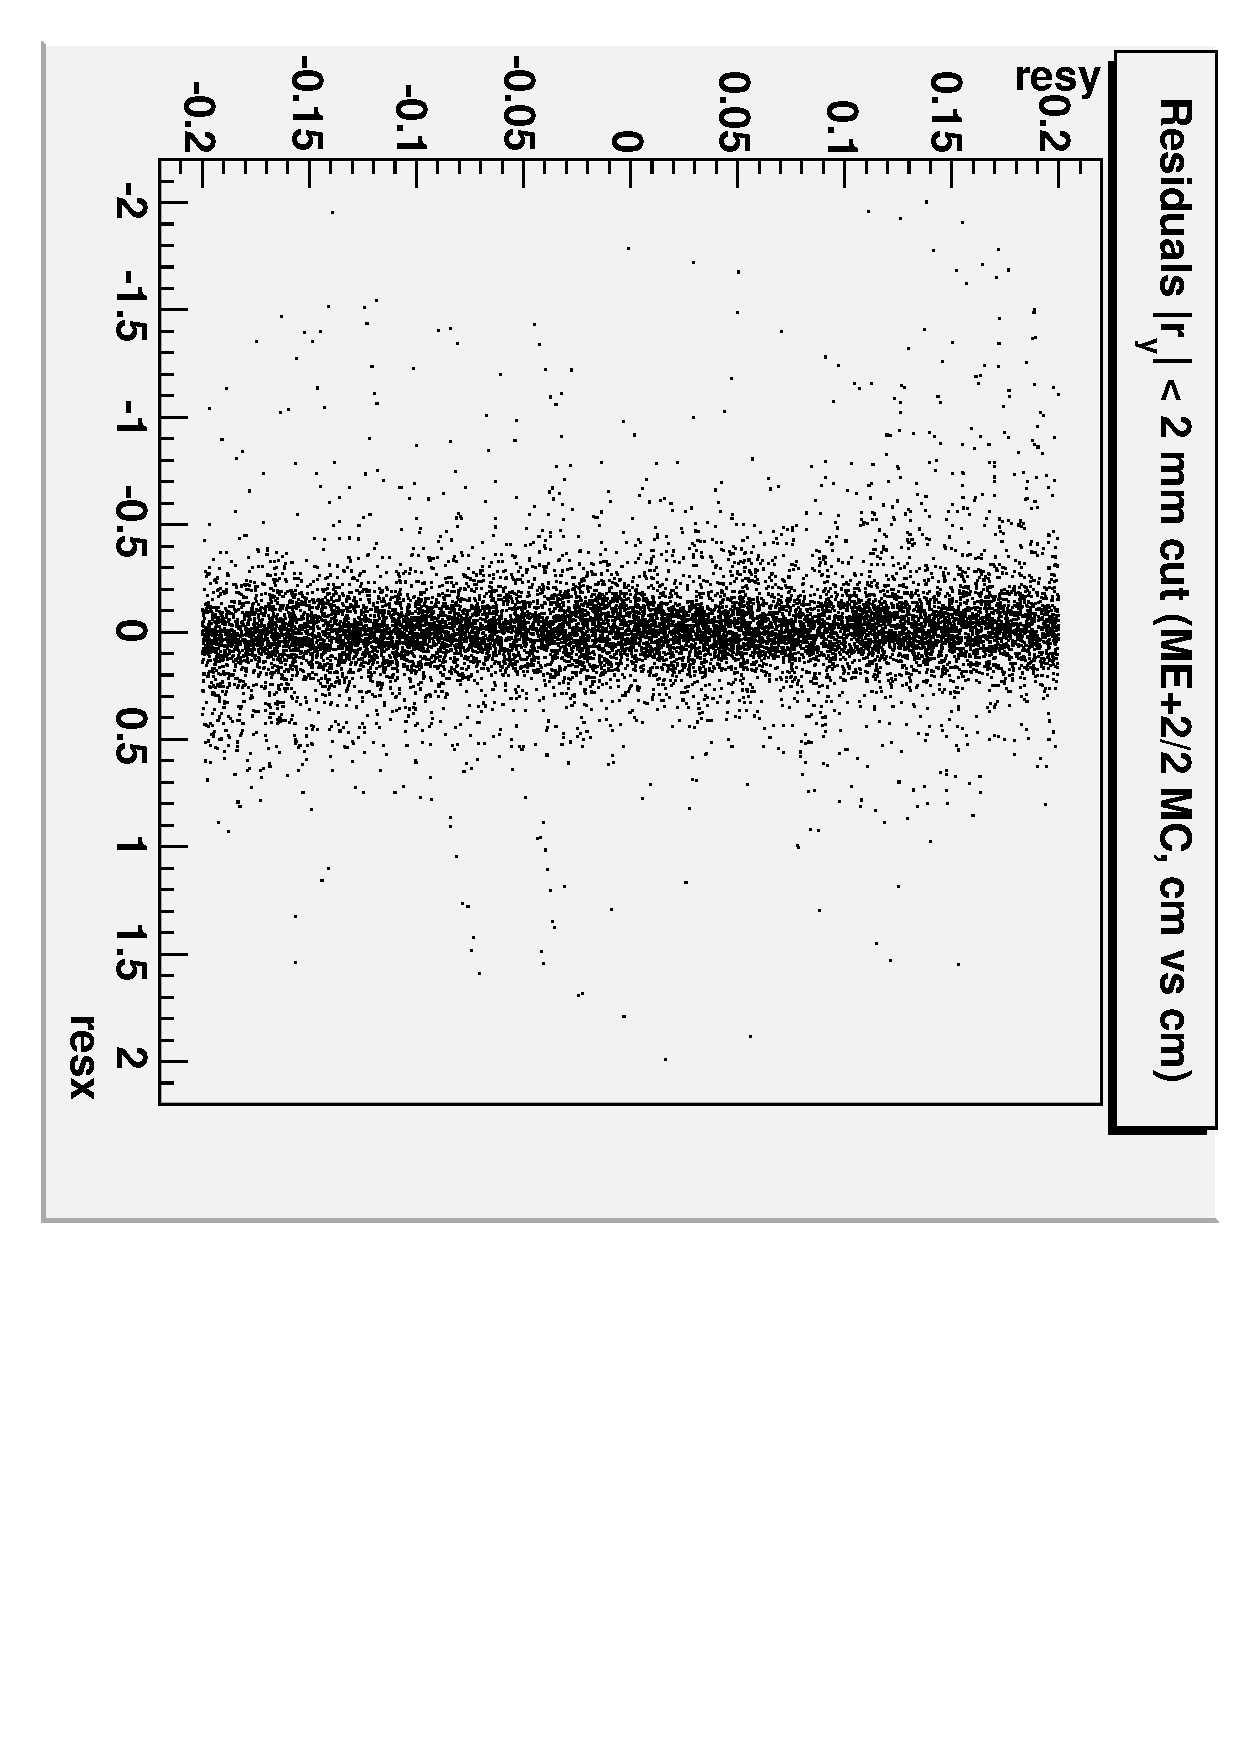
\includegraphics[height=\linewidth, angle=90]{MC_residuals_detail2.pdf}
\column{0.5\linewidth}
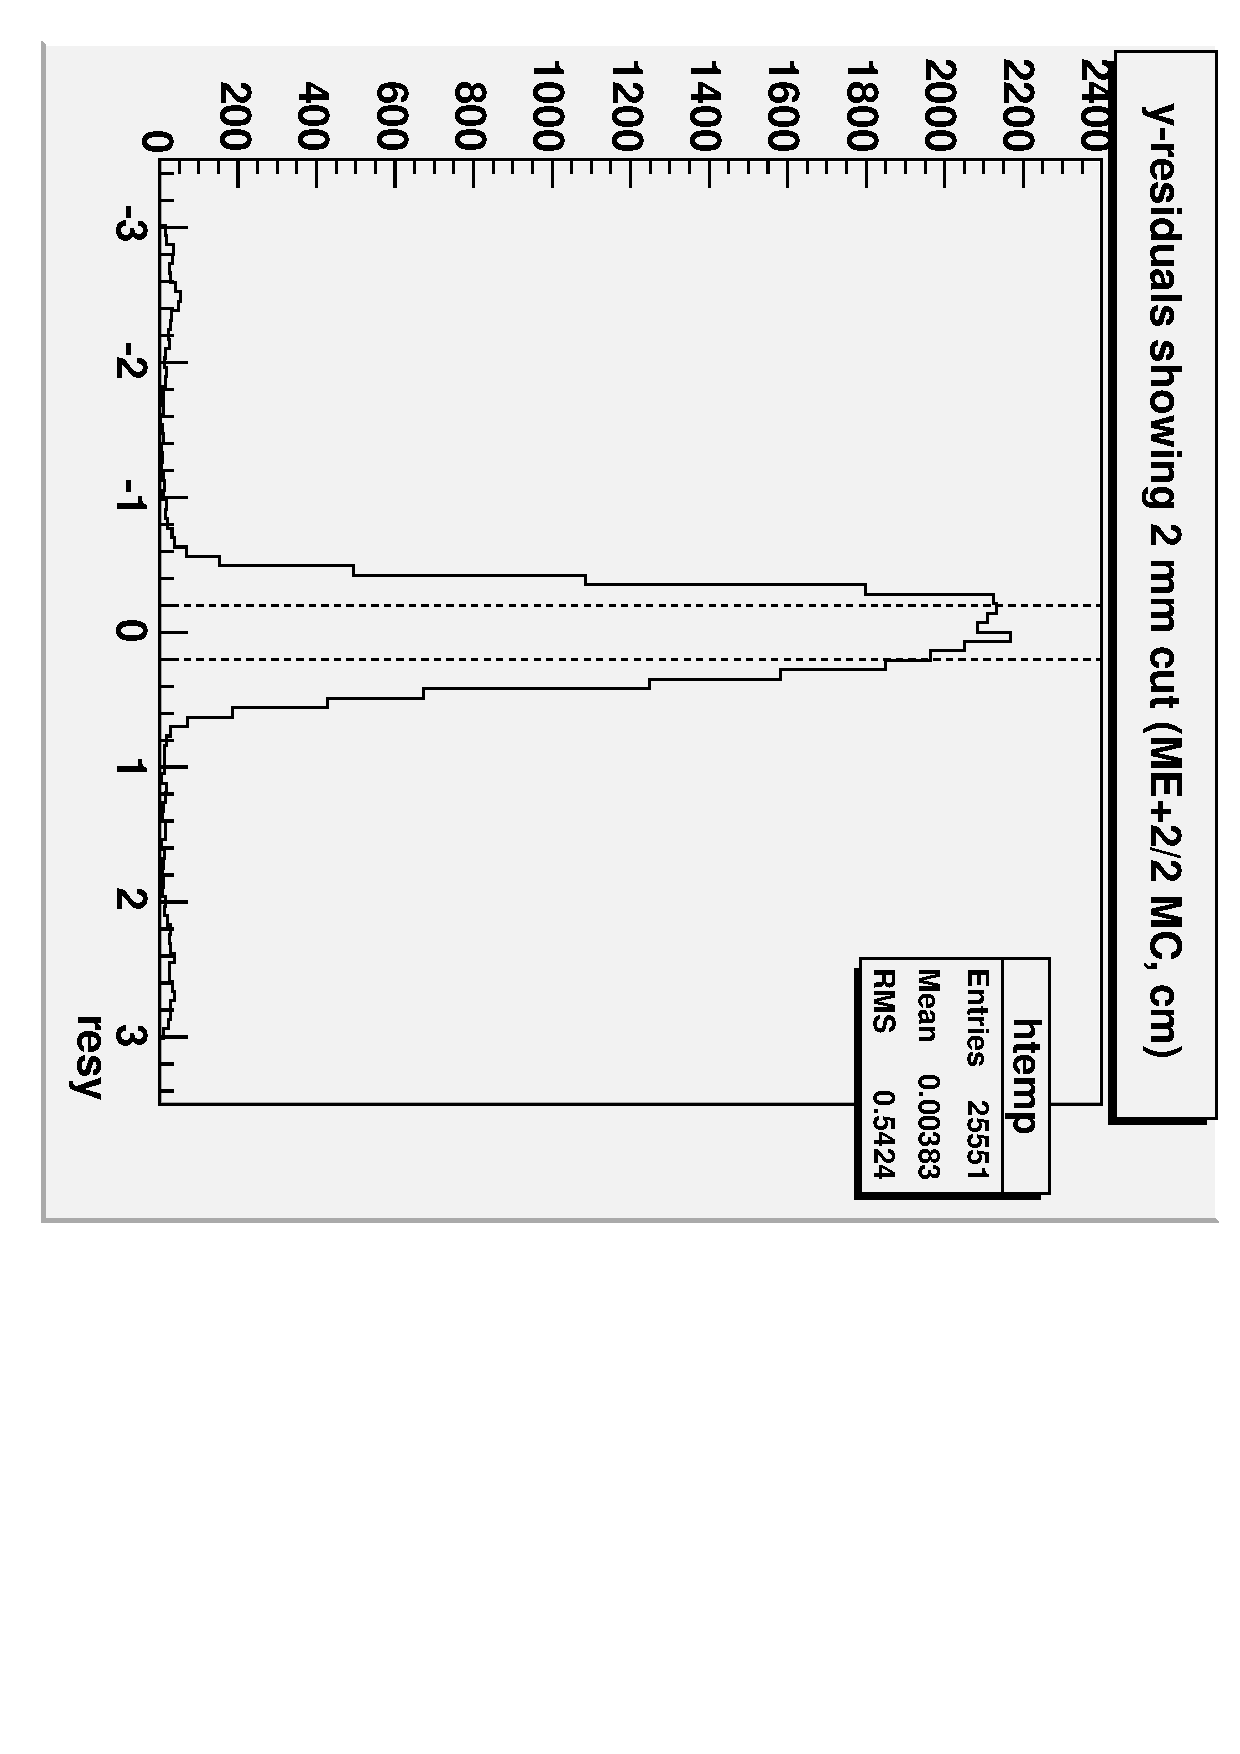
\includegraphics[height=\linewidth, angle=90]{MC_residuals_detail2-yprojection.pdf}
\end{columns}
\end{frame}

\begin{frame}
\frametitle{Granularity in beam-halo (2/2)}
\scriptsize

\begin{itemize}
\item Lose a factor of 2, but $x$ residuals become cleaner, better understood
\item Resolution: (half $y$-gap) $\times$ slope $\oplus$ intrinsic = $\frac{\mbox{5~cm}}{2}$ $\times$ 0.1 $\oplus$ 300~$\mu$m = \mbox{2.5~mm \hspace{-1 cm}}
\item Can't do better than this in $x$ because
\begin{columns}
\column{0.01\linewidth}
\mbox{ }

\column{0.6\linewidth}
\begin{itemize}\setlength{\itemsep}{-0.1 cm}
\item \scriptsize we have no knowledge about $y$ except that it's closest to this wire-group center
\item \scriptsize determining $x$ from the strip measurement is a linear function of $y$
\item \scriptsize hmmm\ldots\ why isn't the $x$ residual distribution a rounded box?
\end{itemize}
\column{0.4\linewidth}
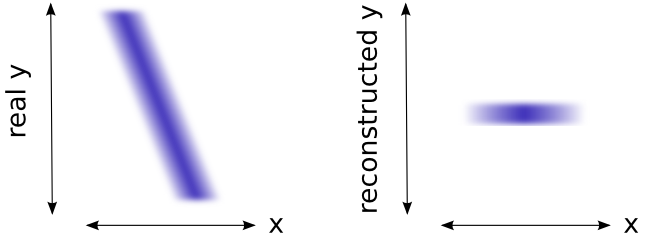
\includegraphics[width=\linewidth]{ignorance_of_y.png}
\end{columns}
\end{itemize}

\vfill
\begin{columns}
\column{0.4\linewidth}
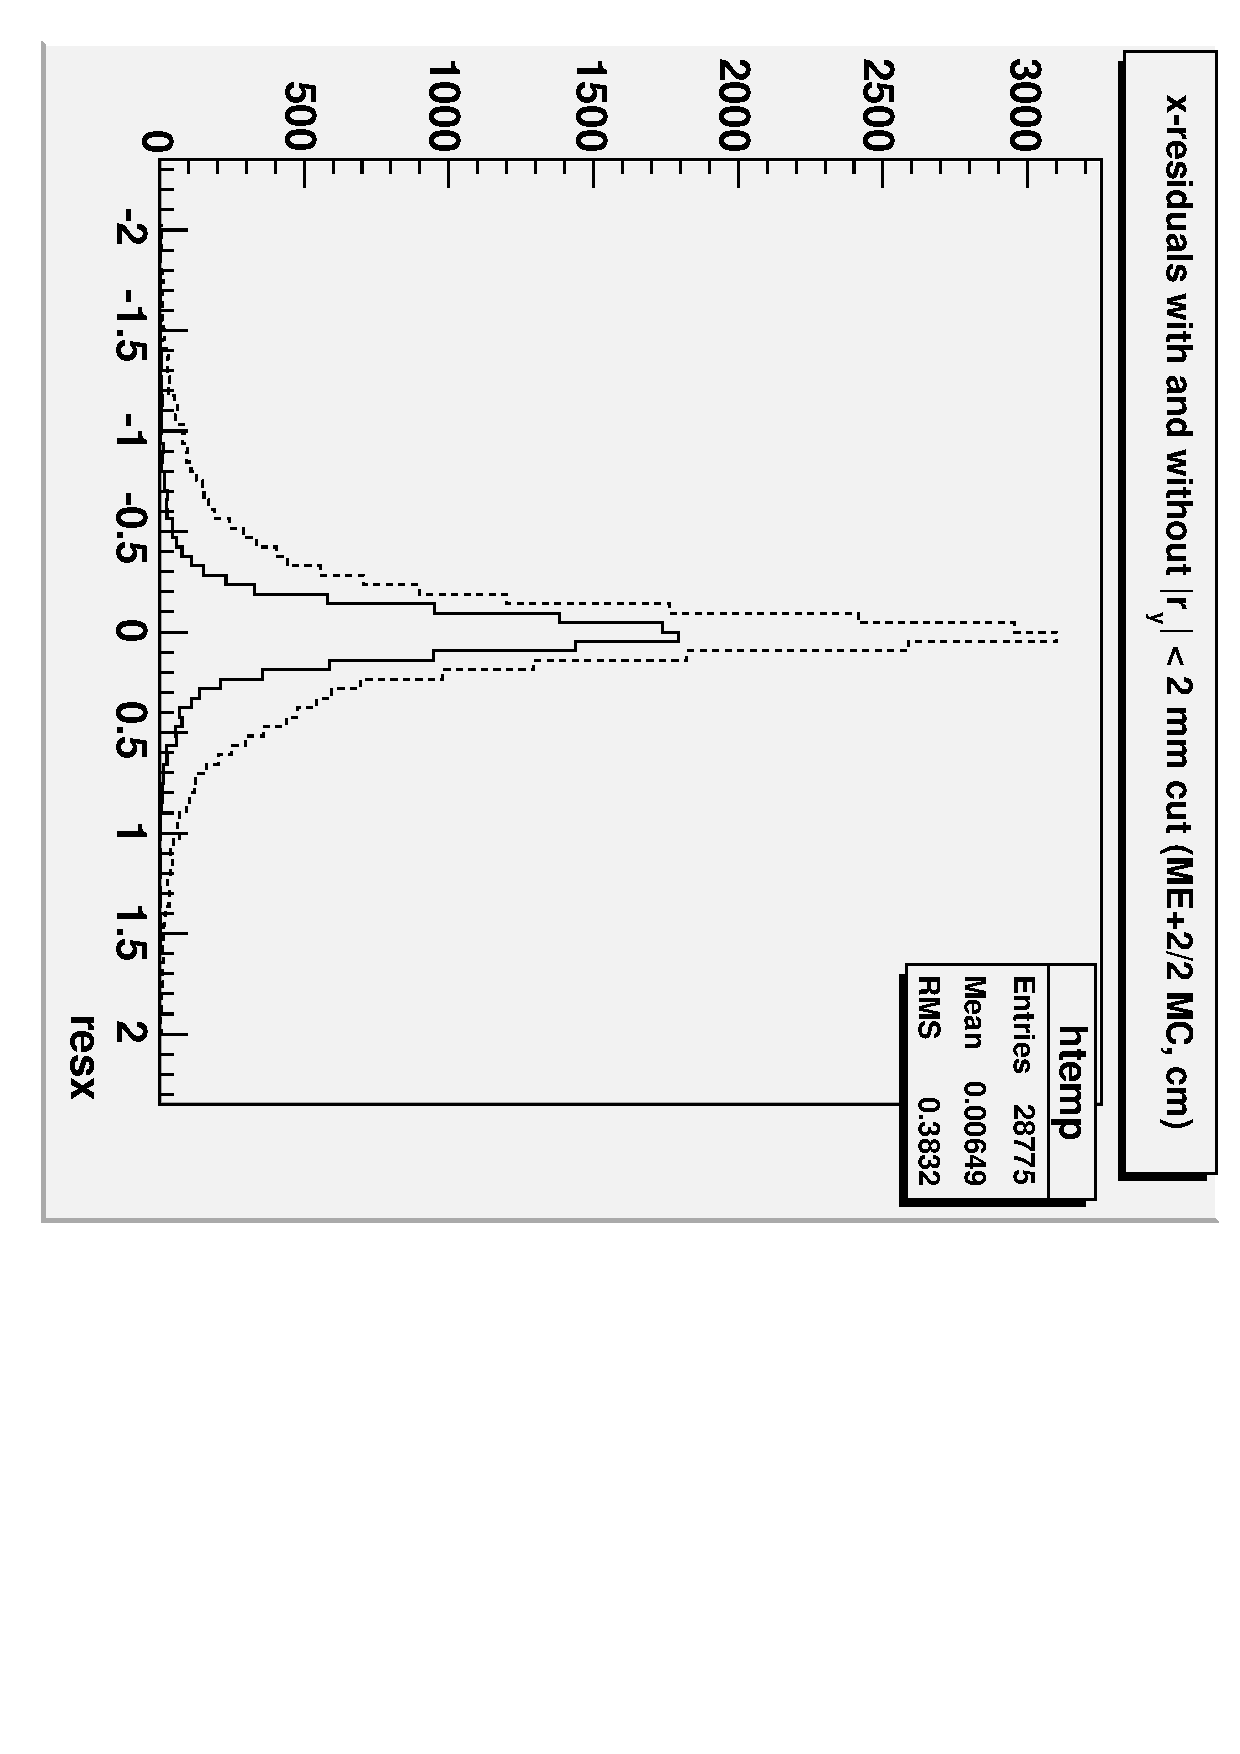
\includegraphics[height=\linewidth, angle=90]{MC_residuals_detail2-xprojection.pdf}
\column{0.6\linewidth}
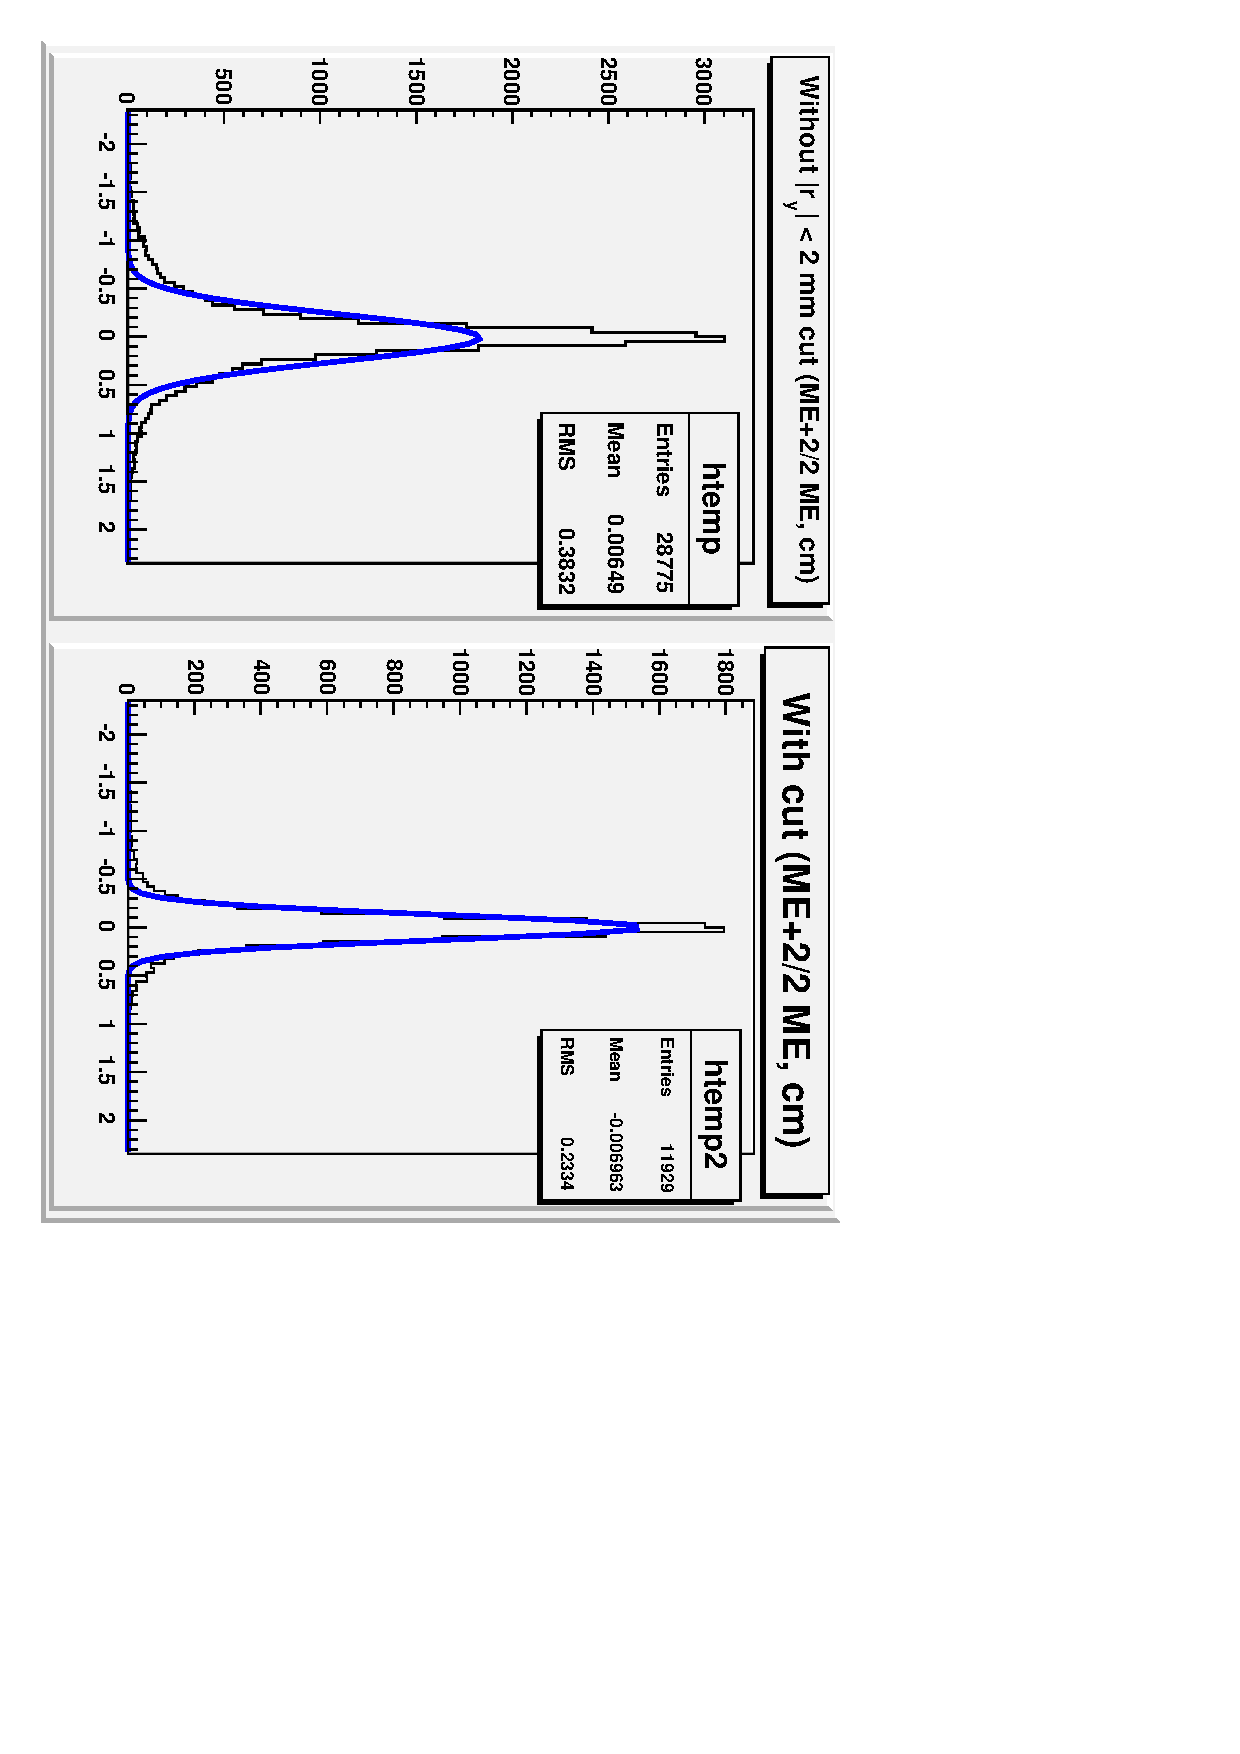
\includegraphics[height=\linewidth, angle=90]{MC_residuals_detail2-xprojection-fits.pdf}
\end{columns}
\end{frame}

\begin{frame}
\frametitle{Inner ring vs.\ outer ring}
\scriptsize
\begin{itemize}
\item Wire groups are 1.6~cm apart in ME+2/1, as opposed to 5~cm
\item Smaller spacing washes out structure; harder to see $\pm$0, $\pm$1\ldots, peaks
\item Slope in $x$-$y$ correlation is 0.35, consistent with 20$^\circ$ trapezoidal chamber design
\end{itemize}

\vfill
\begin{columns}
\column{0.3\linewidth}
$y$ hit position histograms

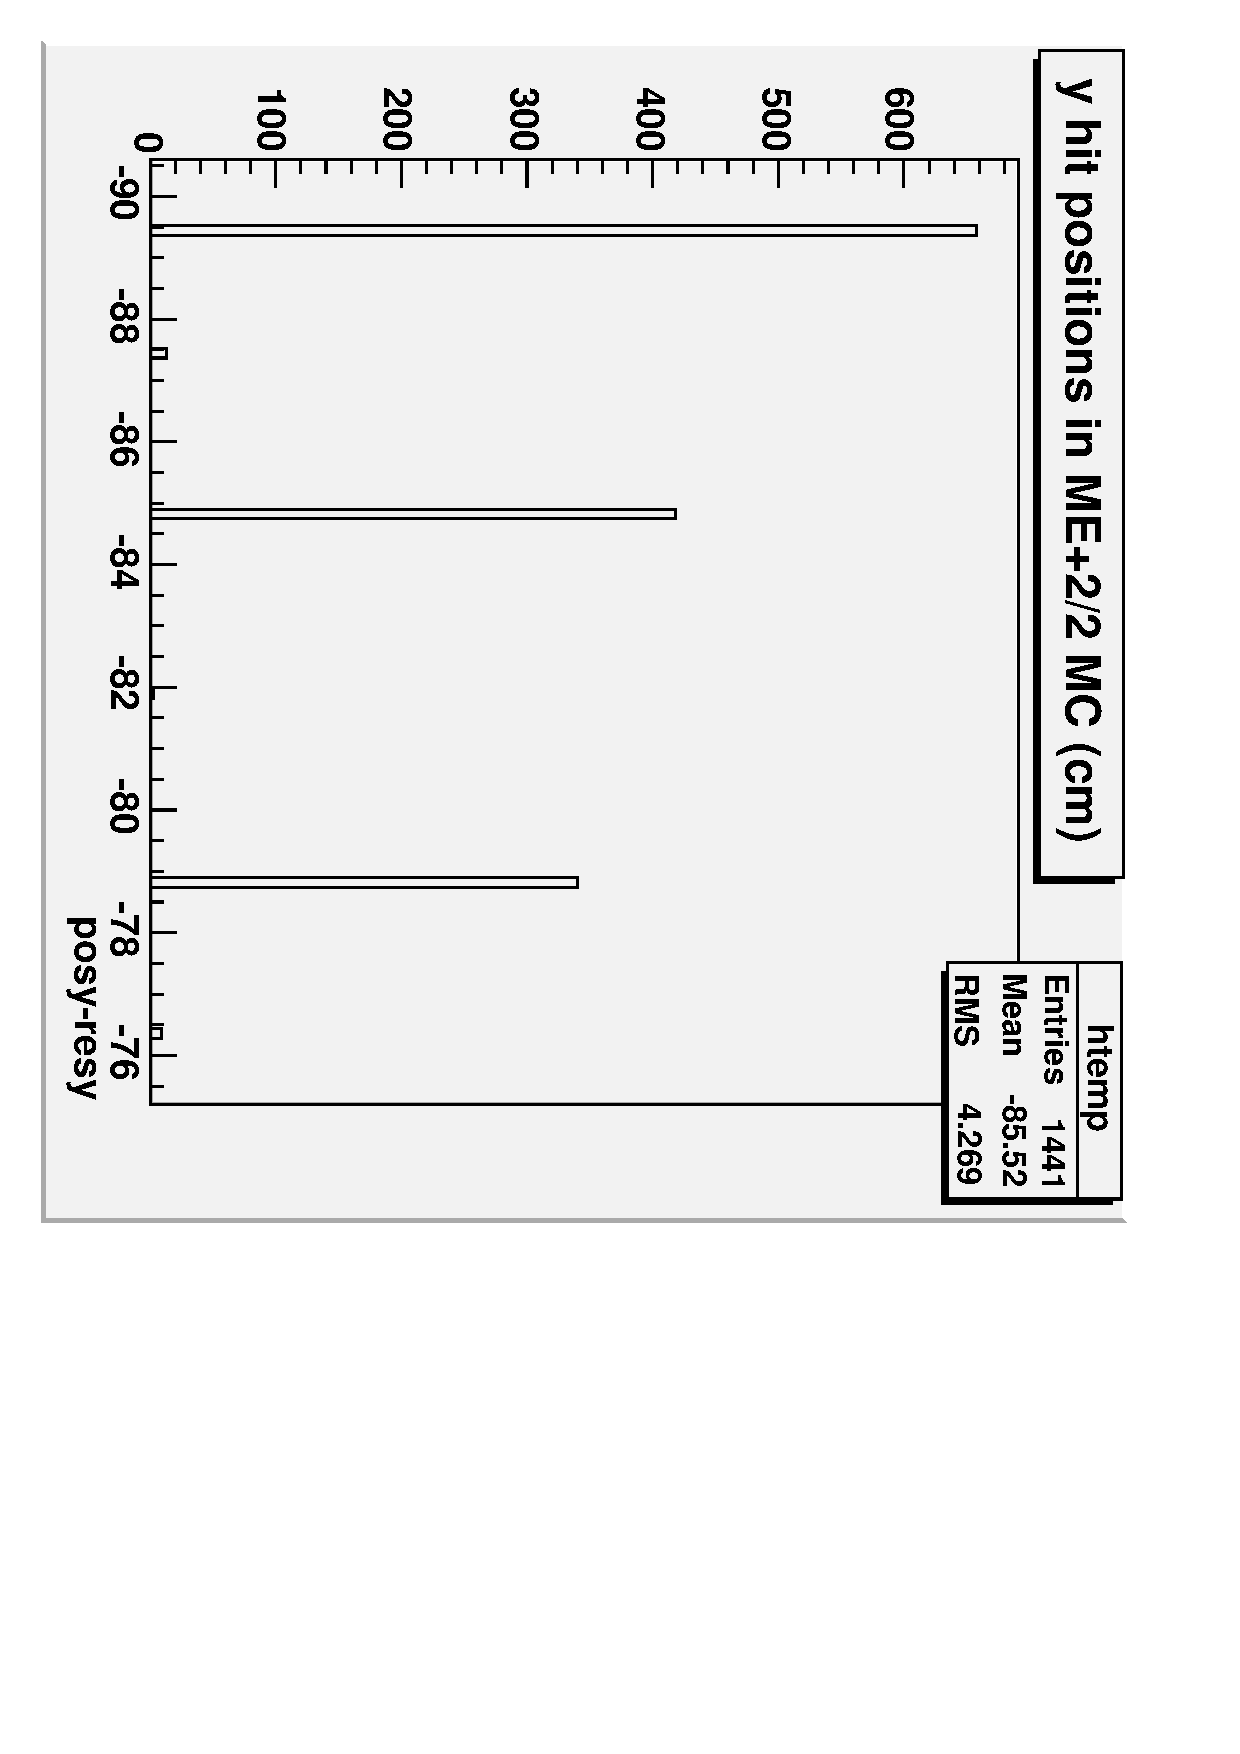
\includegraphics[height=\linewidth, angle=90]{MC_y_hits_detail.pdf}
\column{0.3\linewidth}
same window width

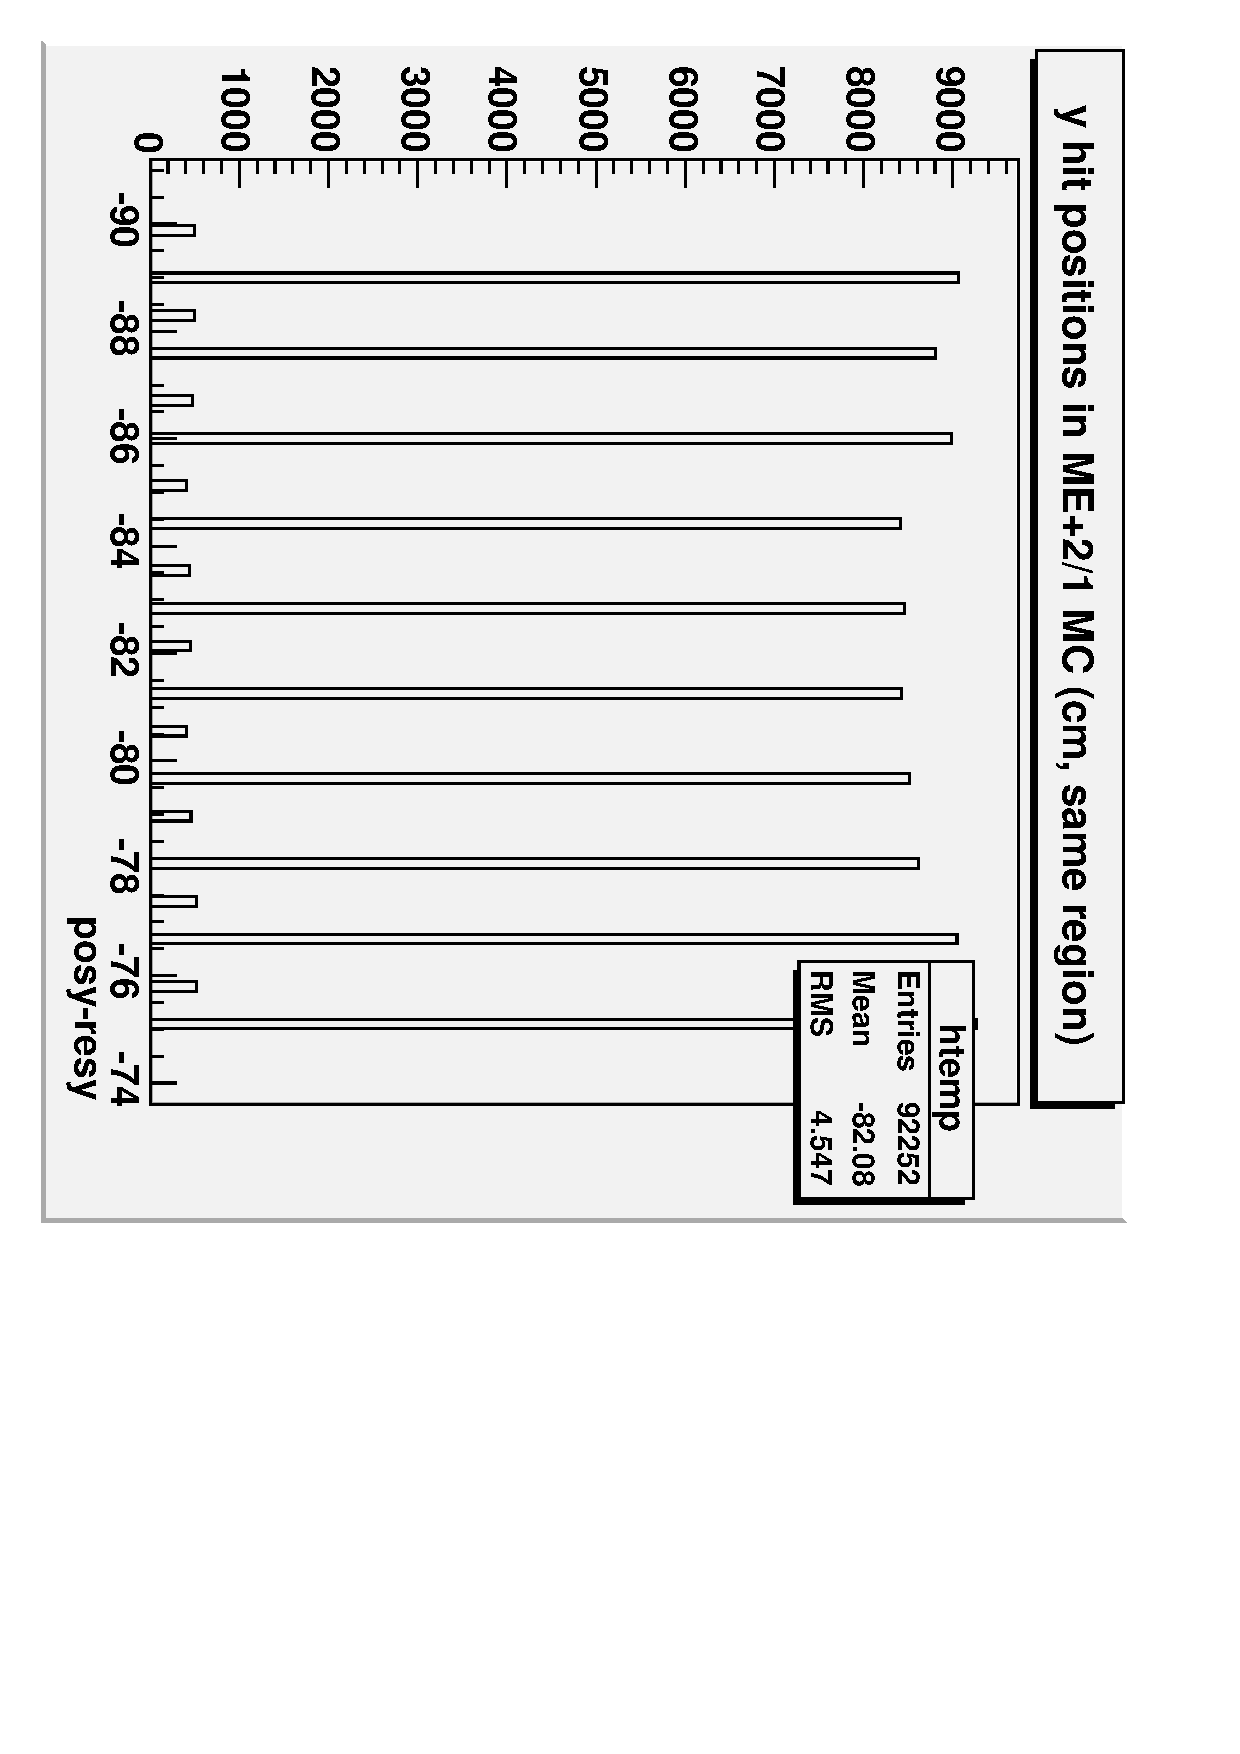
\includegraphics[height=\linewidth, angle=90]{MC_y_hits_detail2.pdf}
\column{0.5\linewidth}
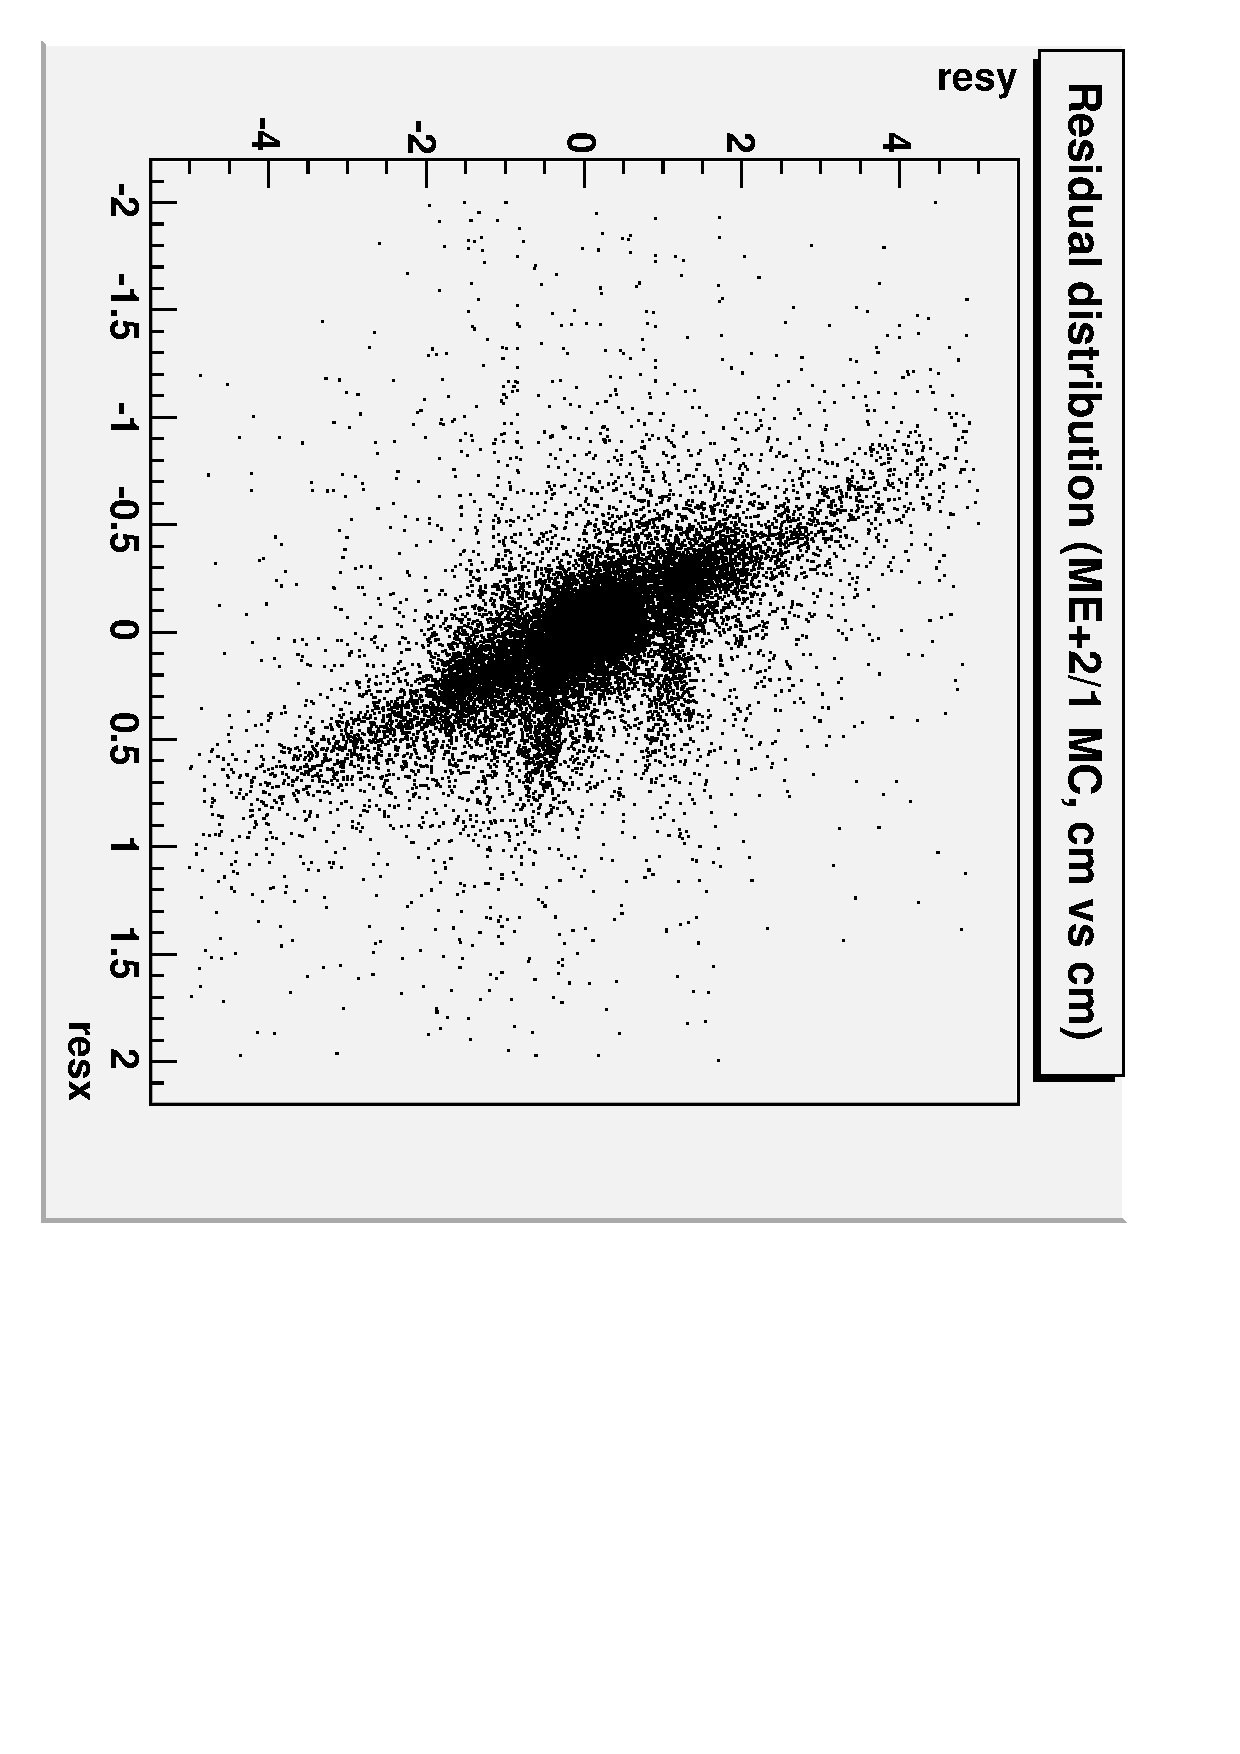
\includegraphics[height=\linewidth, angle=90]{MC_residuals_ME21.pdf}
\end{columns}
\end{frame}

\begin{frame}
\frametitle{Same trick in inner ring}
\scriptsize
\begin{itemize}
\item Much greater loss in statistics due to greater probability of $\Delta y$ = 1 or 2
\item Only a marginal benefit, but final resolution is the same: (half~$y$-gap)~$\times$~slope~=~$\frac{\mbox{1.6 cm}}{2}$~0.35~=~2.5~mm (by design?)
\item When $y$ is very granular, it pays to take advantage of this and
  select the clean central region, and if $y$ were completely
  continuous, we wouldn't need to do anything special.  But what about the middle case?
\end{itemize}

\vfill
\begin{columns}
\column{0.4\linewidth}
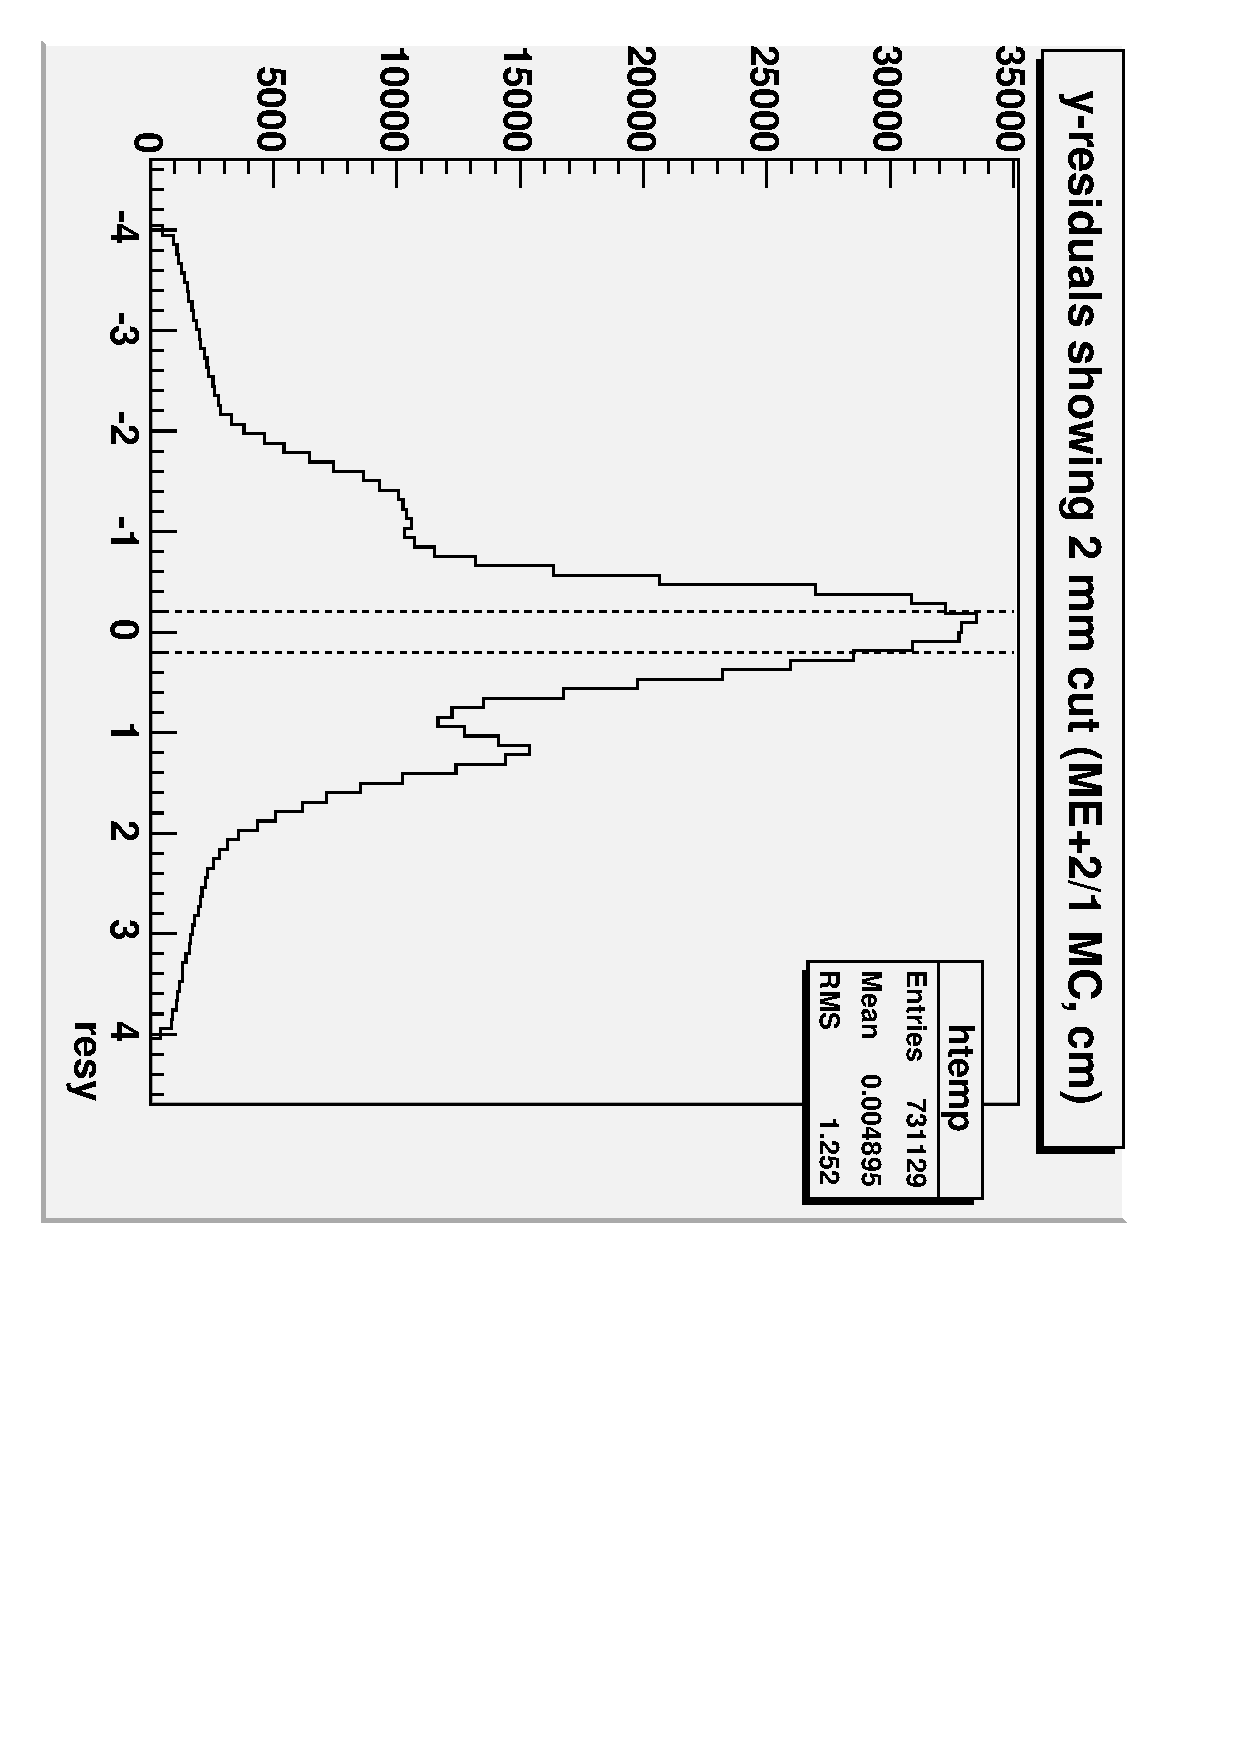
\includegraphics[height=\linewidth, angle=90]{MC_residuals_detail2-yprojection_ME21.pdf}
\column{0.6\linewidth}
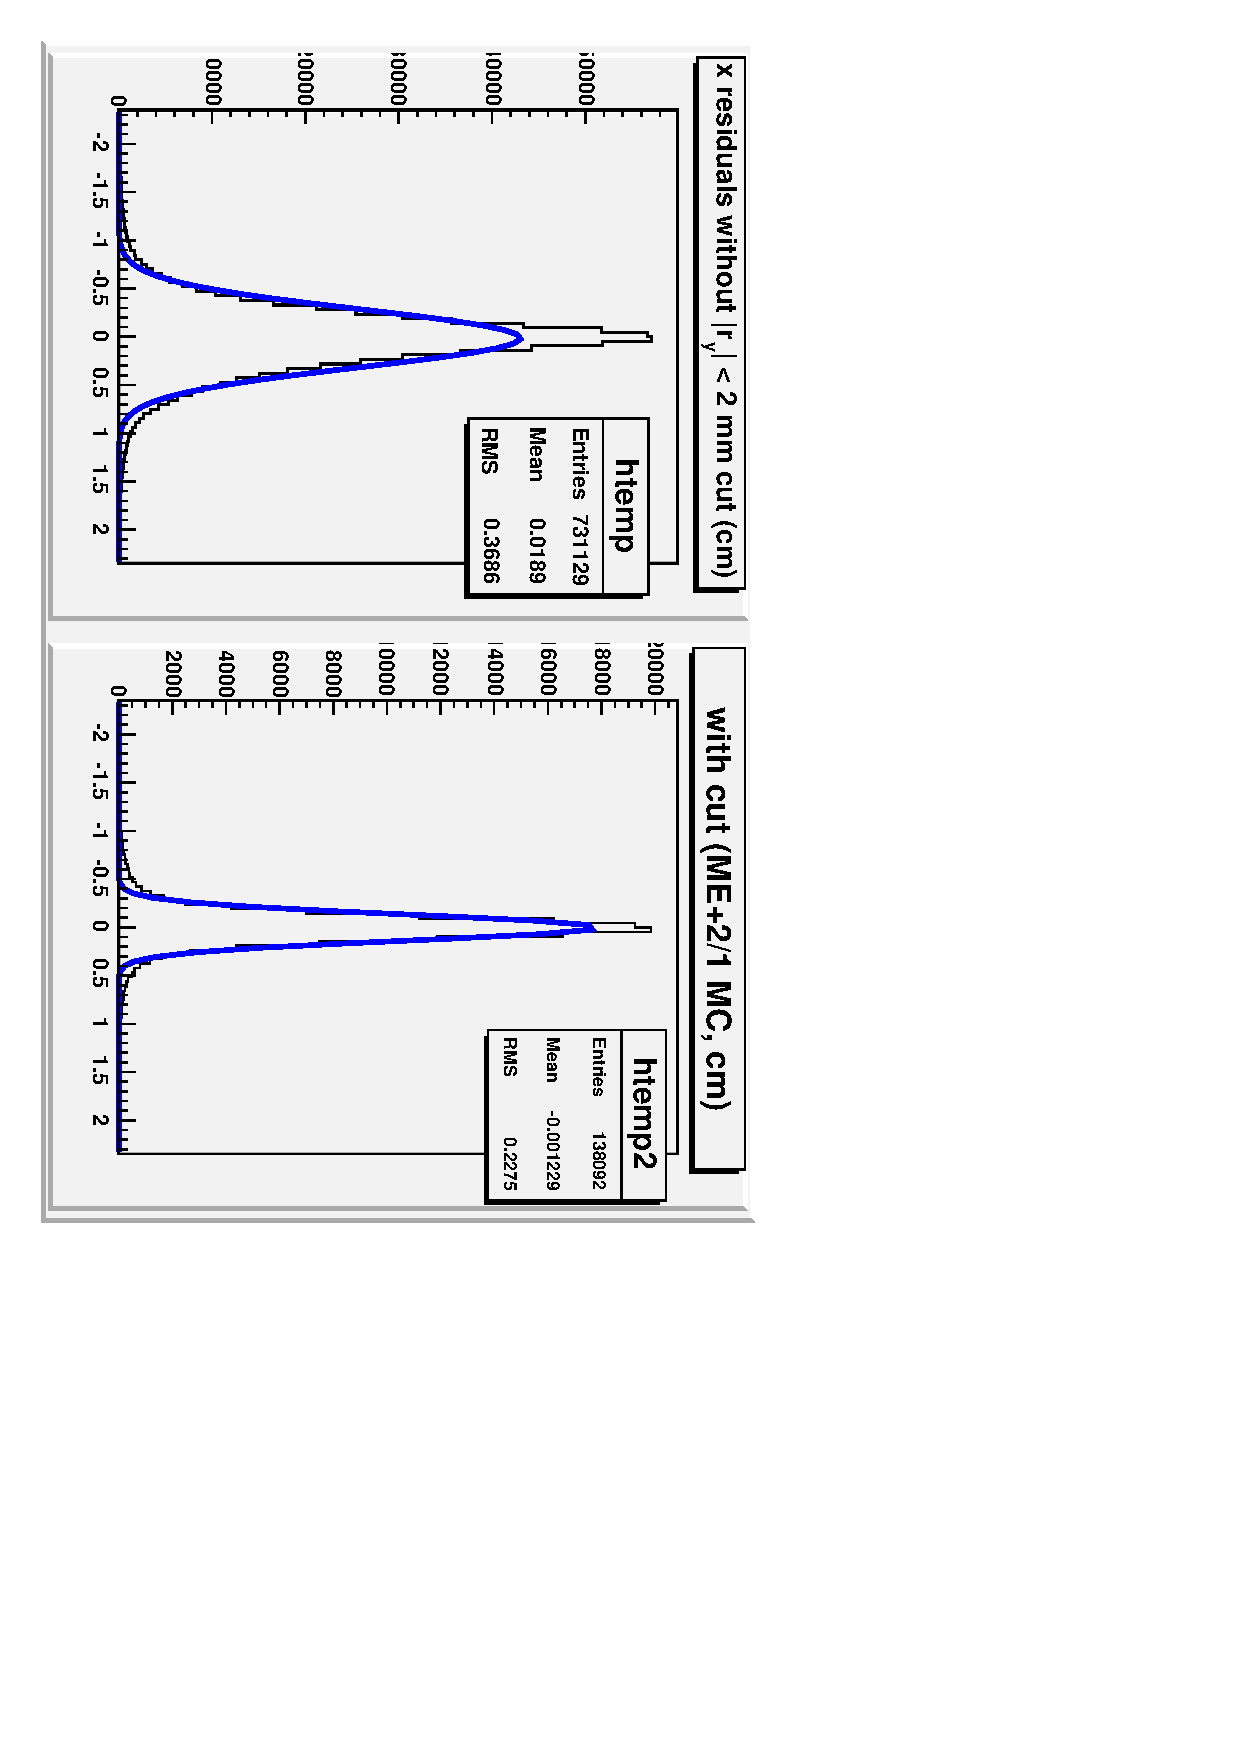
\includegraphics[height=\linewidth, angle=90]{MC_residuals_detail2-xprojection-fits_ME21.pdf}
\end{columns}
\end{frame}

\begin{frame}
\frametitle{Data are smooth}
\scriptsize
\begin{itemize}
\item Like I said, it's the fact that they're cosmic rays with
  non-horizontal impact angles (and the fact that there's a spread in
  impact angles can only help)
\item Cutting central region trick does very little good here
\item The distribution looks smooth: do you suppose it really is
  smooth?  Can we just assume that the Gaussian correlations-handling
  in HIPAlignmentAlgorithm will take care of it?
\item Layer misalignments can also smooth the $y$ residuals, but 6 is
  a rather small number for such featurelessness
\item Alignment artifacts we see in beam-halo MC will not necessarily
  affect cosmics data, so the MC is not a very helpful guide
\end{itemize}

\vfill
\begin{columns}
\column{0.4\linewidth}
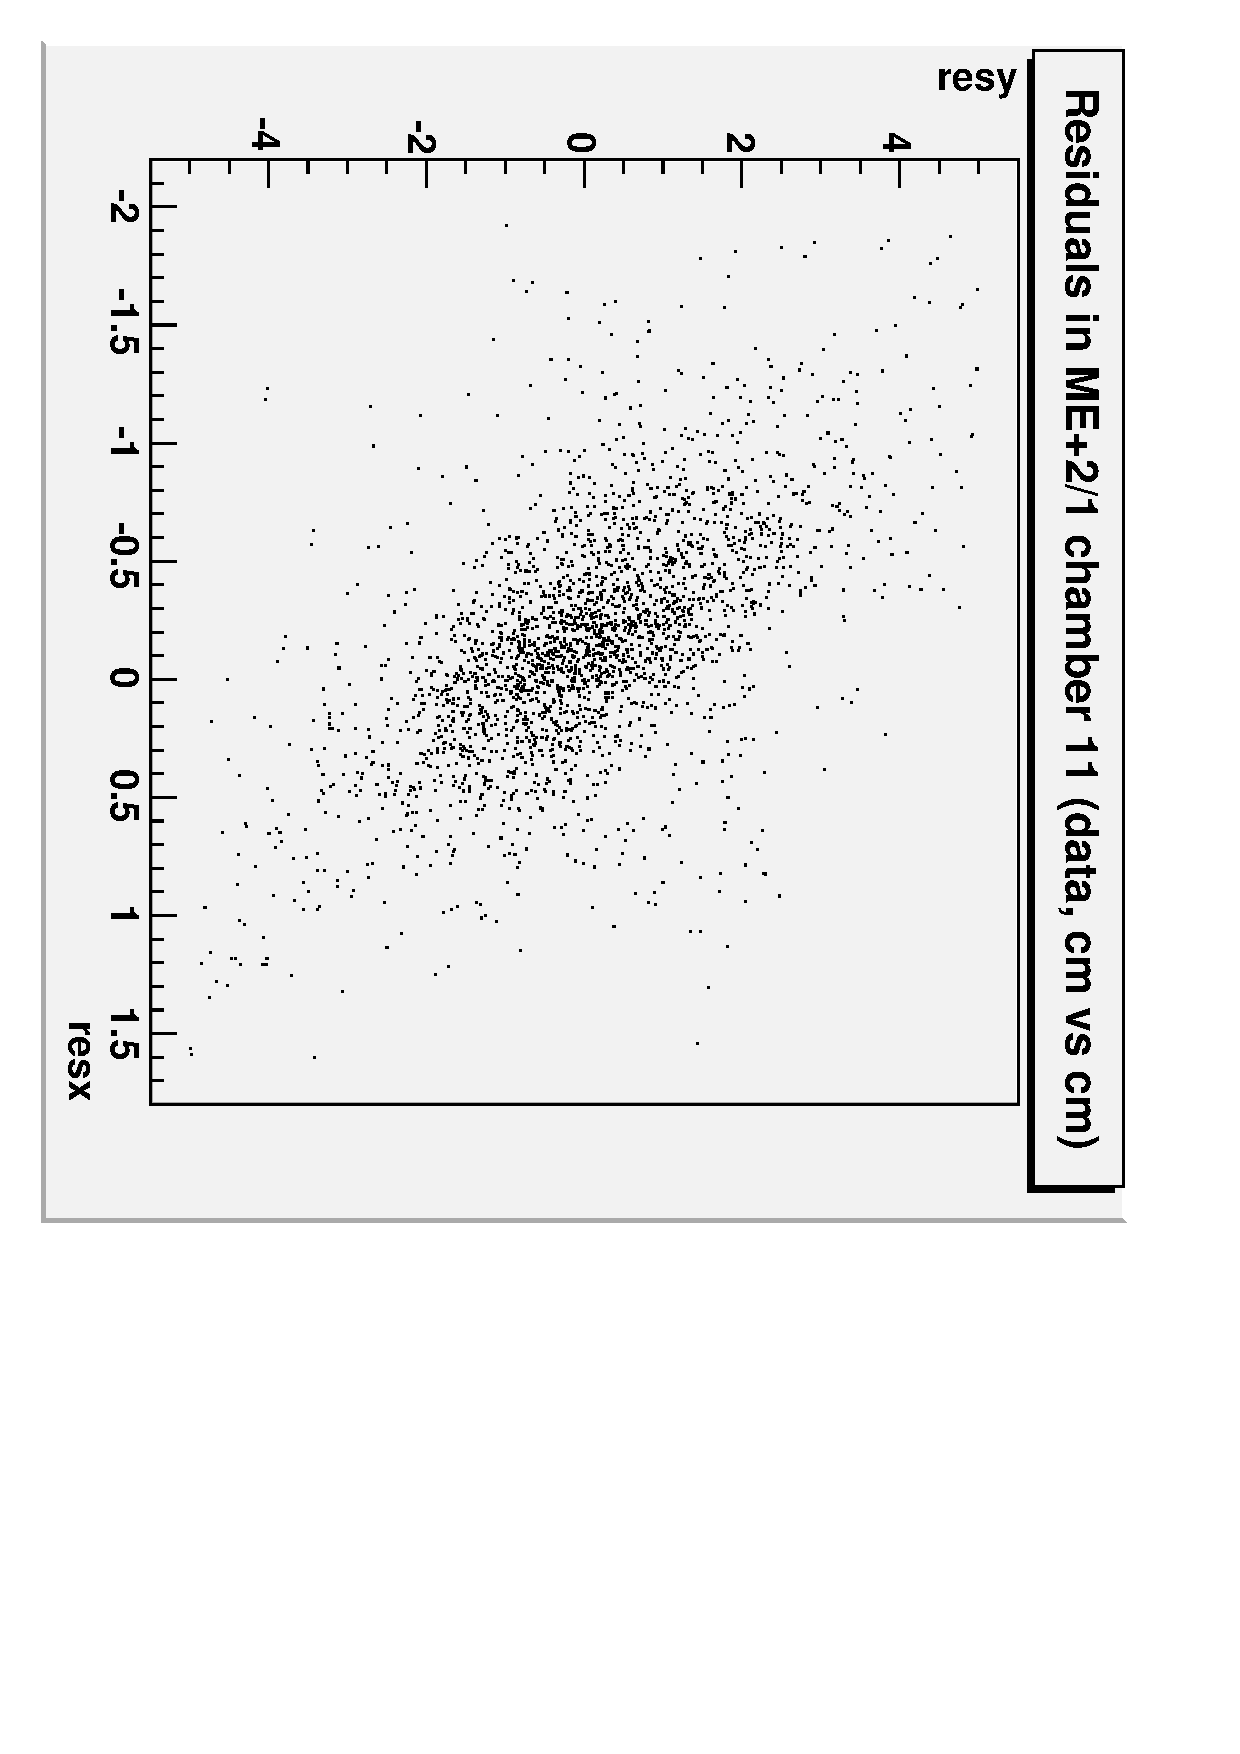
\includegraphics[height=\linewidth, angle=90]{data_residuals_ME21.pdf}
\column{0.6\linewidth}
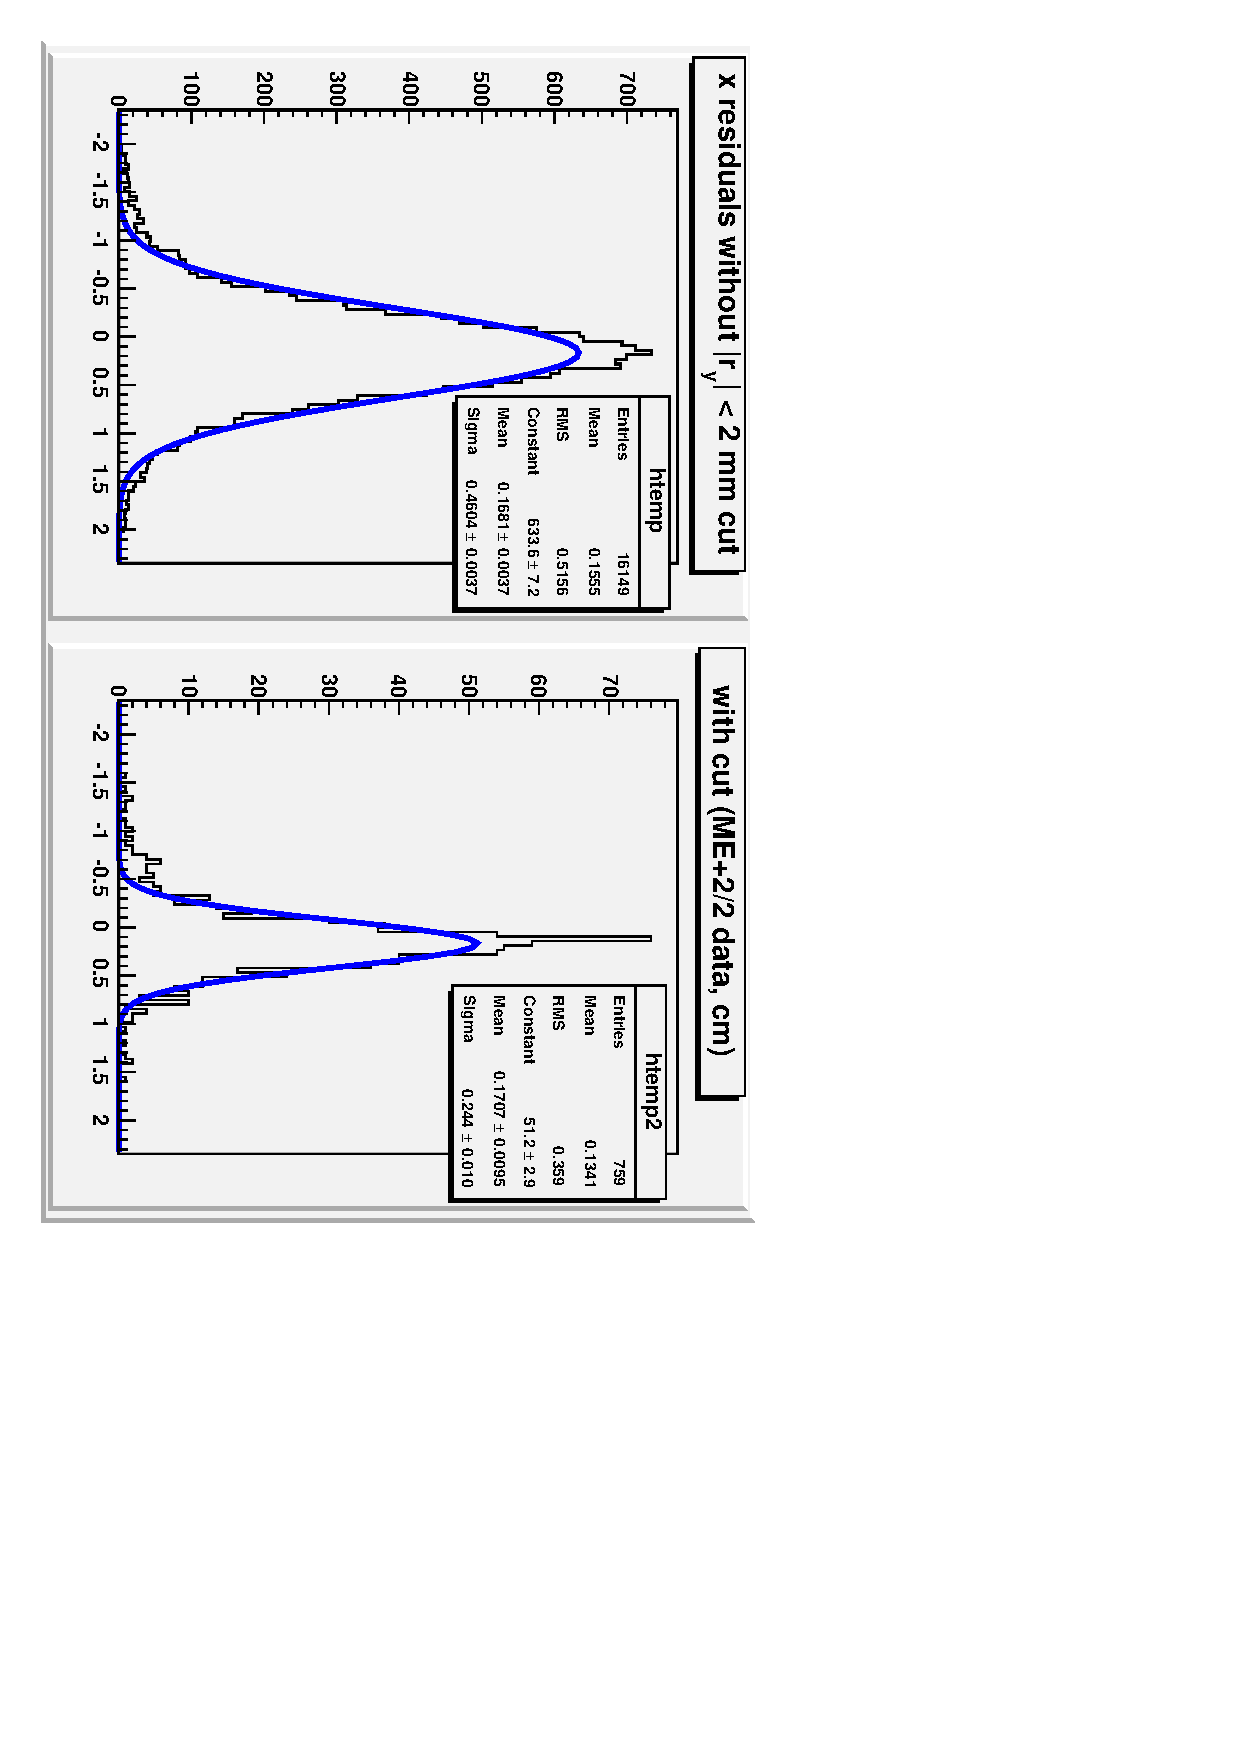
\includegraphics[height=\linewidth, angle=90]{data_residuals_detail2-xprojection-fits_ME22.pdf}
\end{columns}
\end{frame}

\begin{frame}
\frametitle{Occupancies: not very flat}

\begin{columns}
\column{0.4\linewidth}
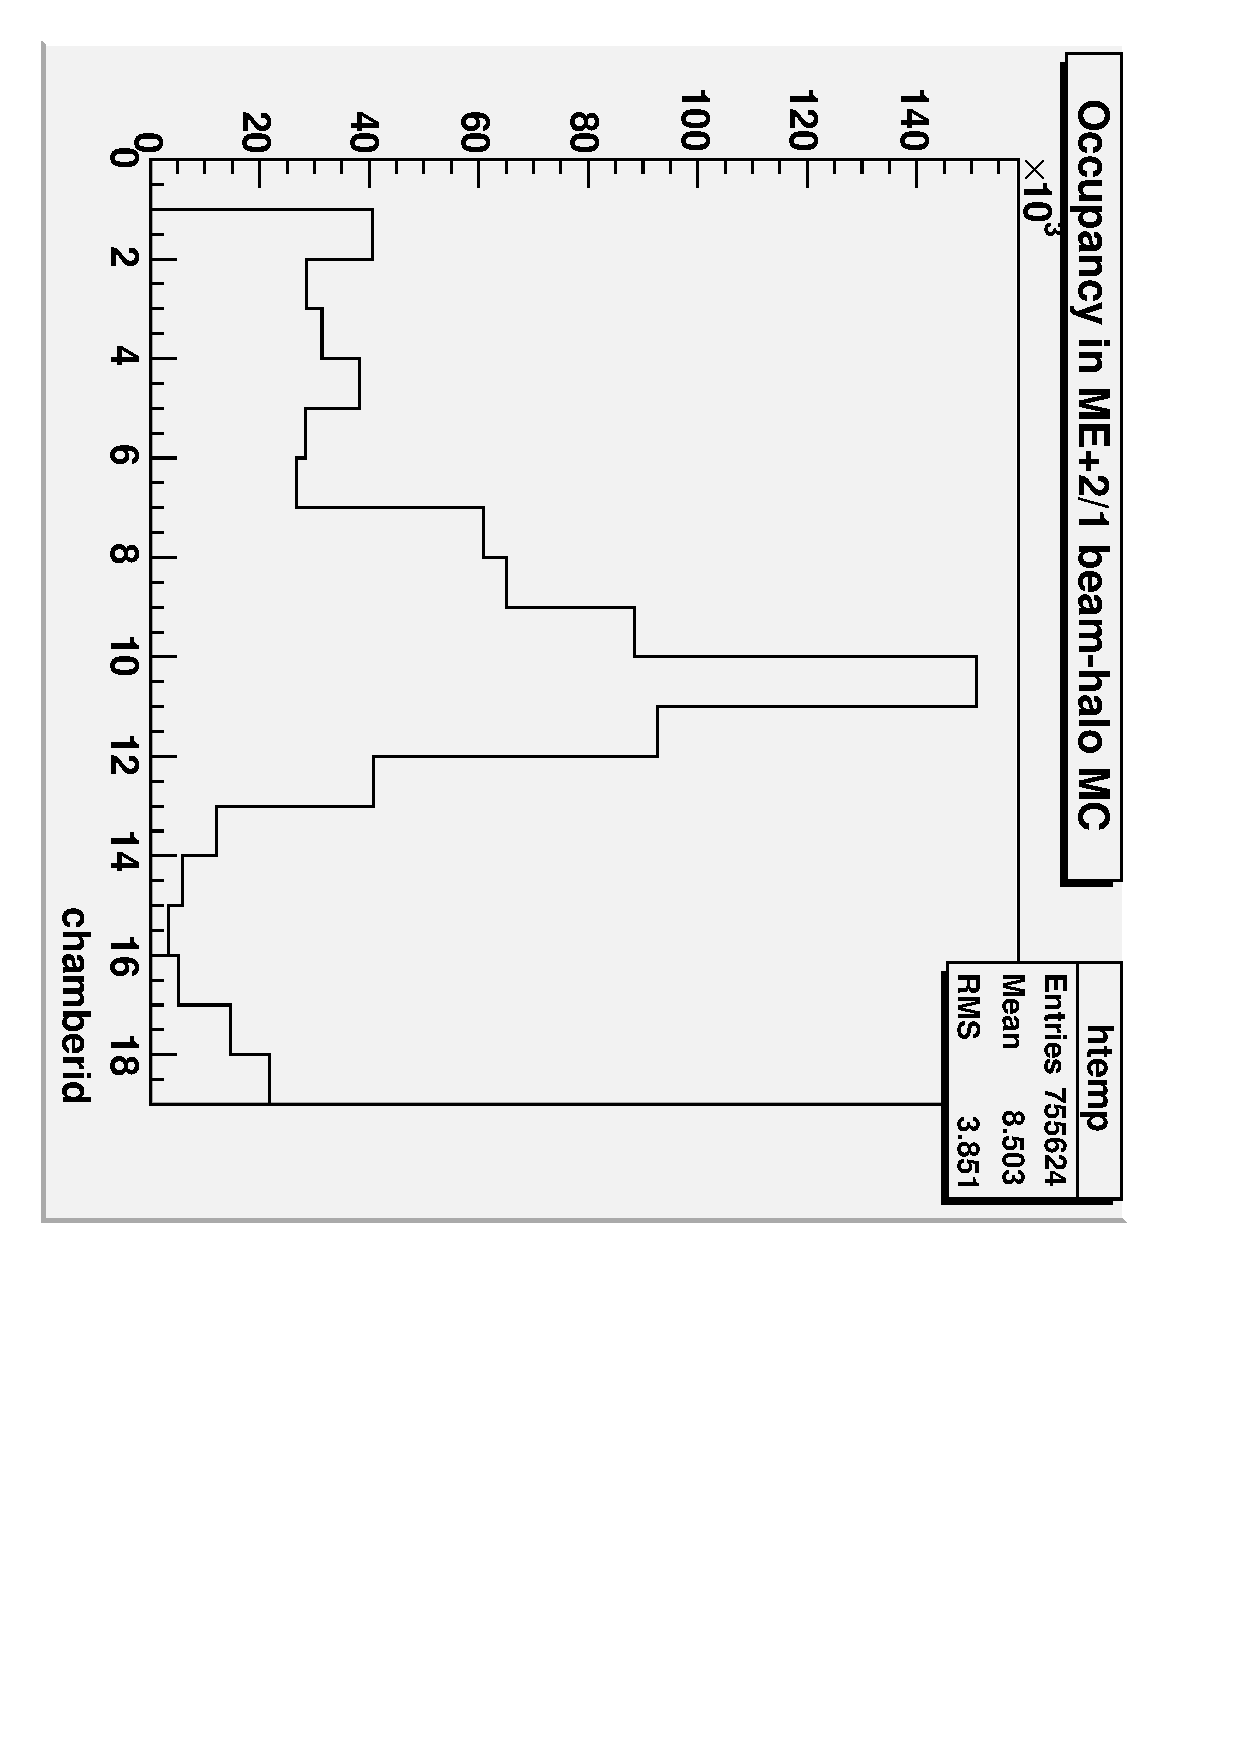
\includegraphics[height=\linewidth, angle=90]{MC_occupancy_ME21.pdf}

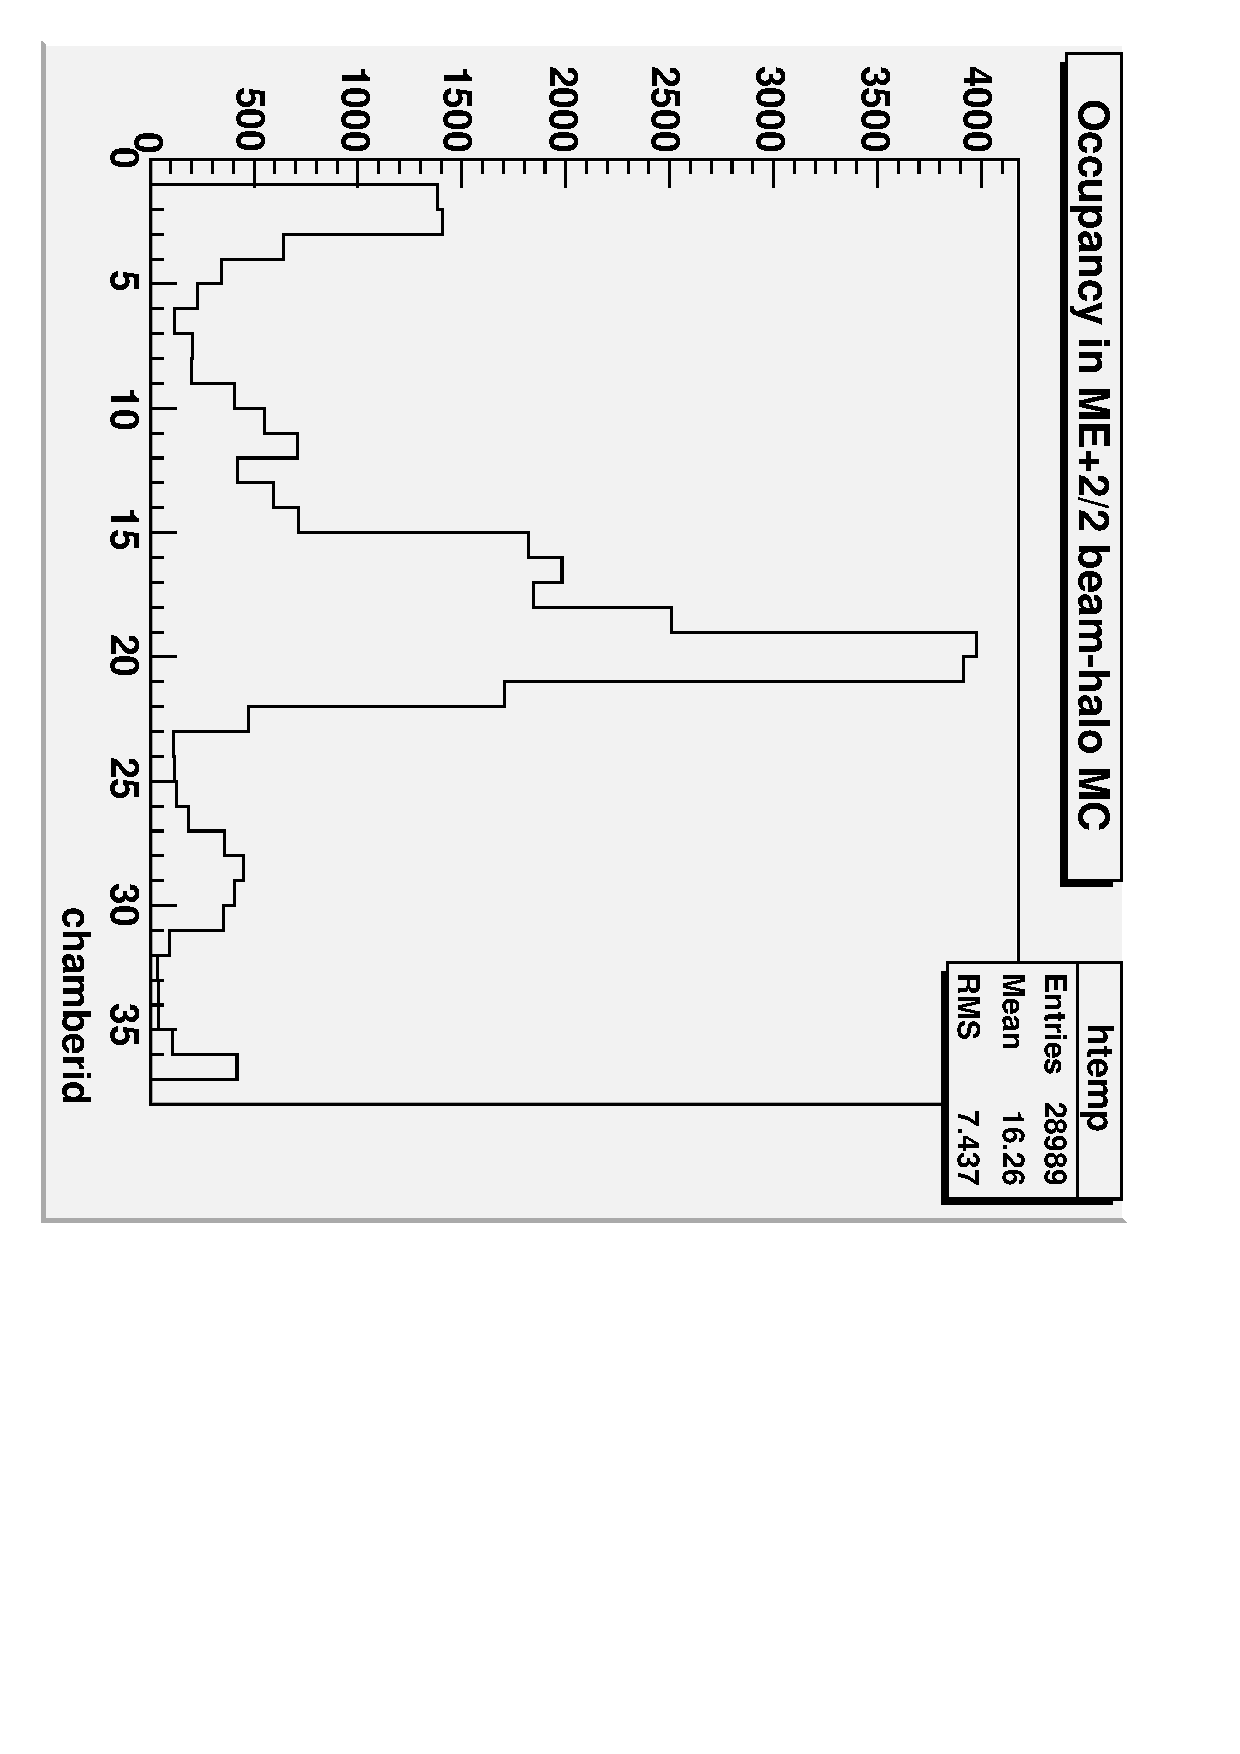
\includegraphics[height=\linewidth, angle=90]{MC_occupancy_ME22.pdf}

\column{0.4\linewidth}
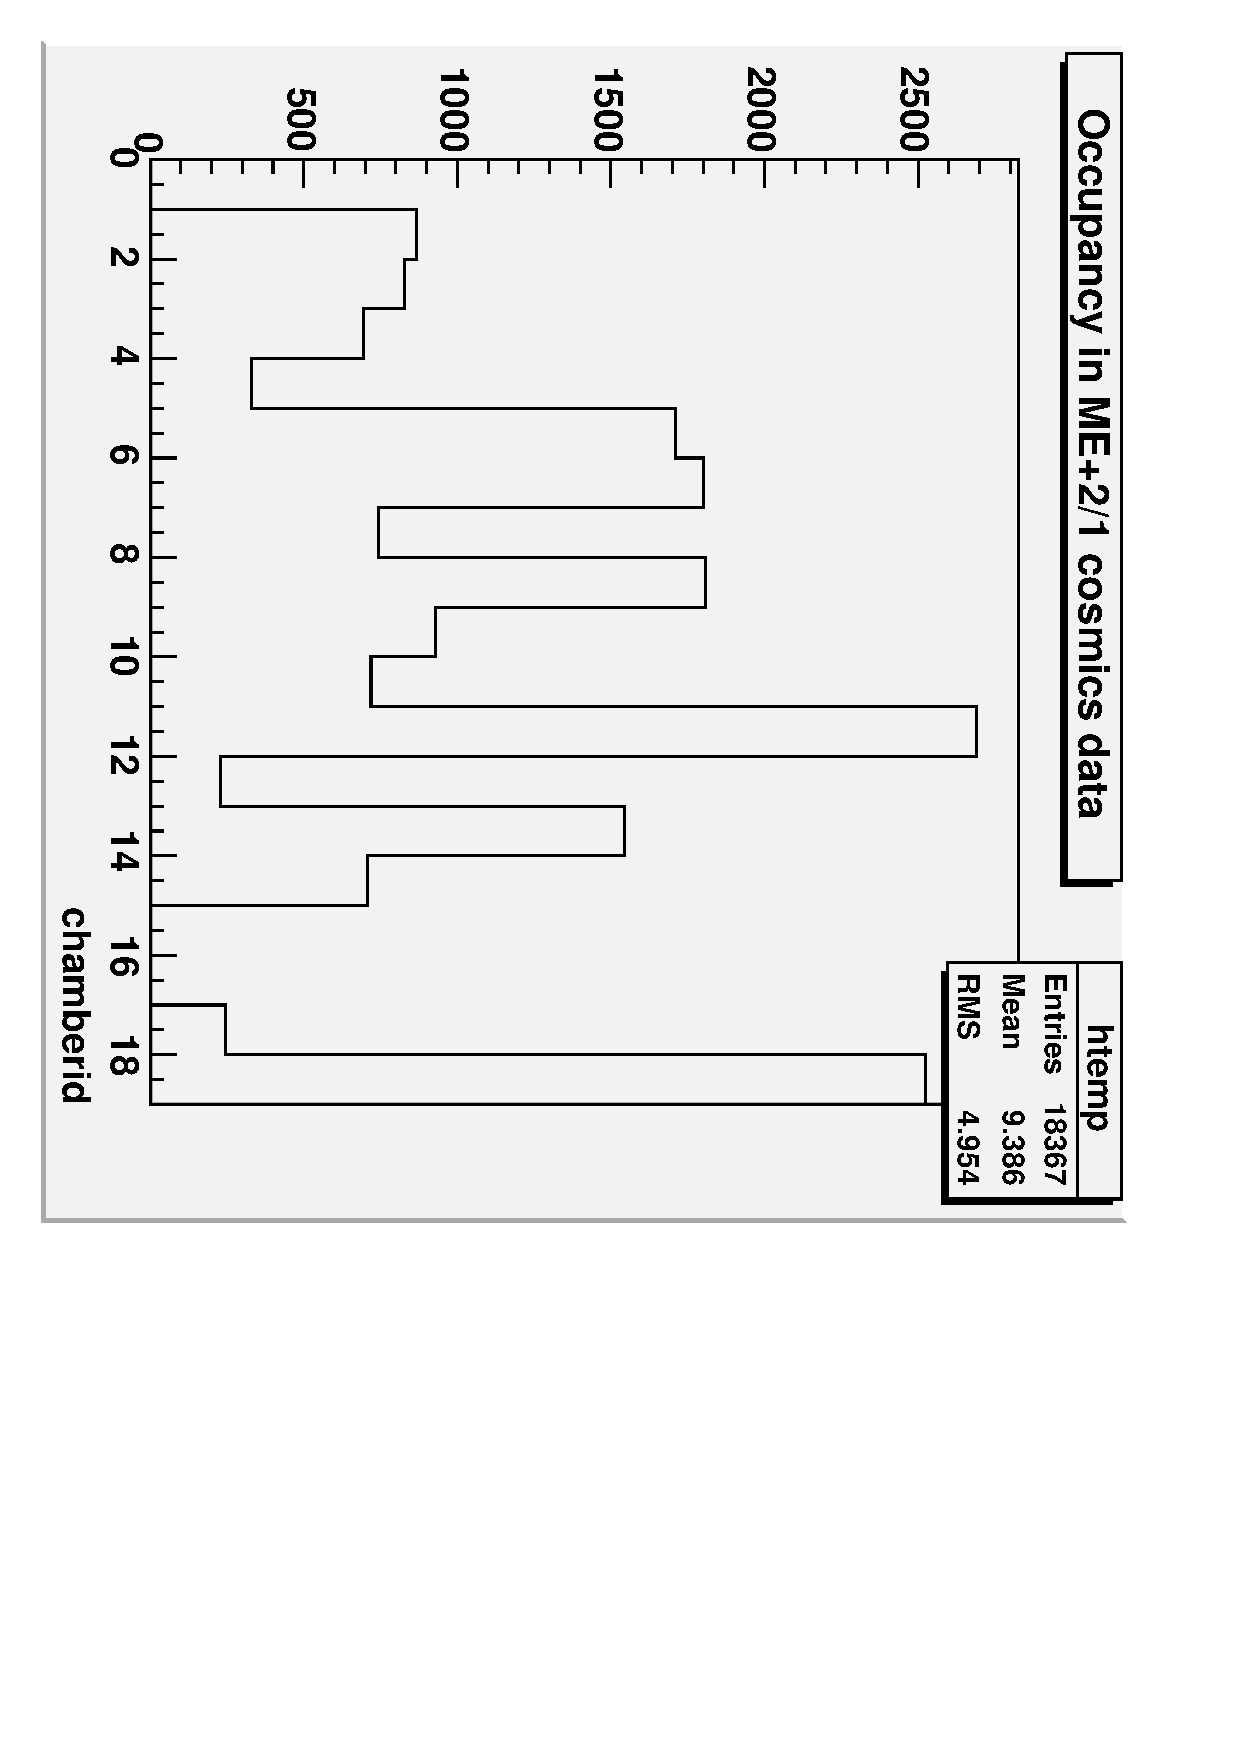
\includegraphics[height=\linewidth, angle=90]{data_occupancy_ME21.pdf}

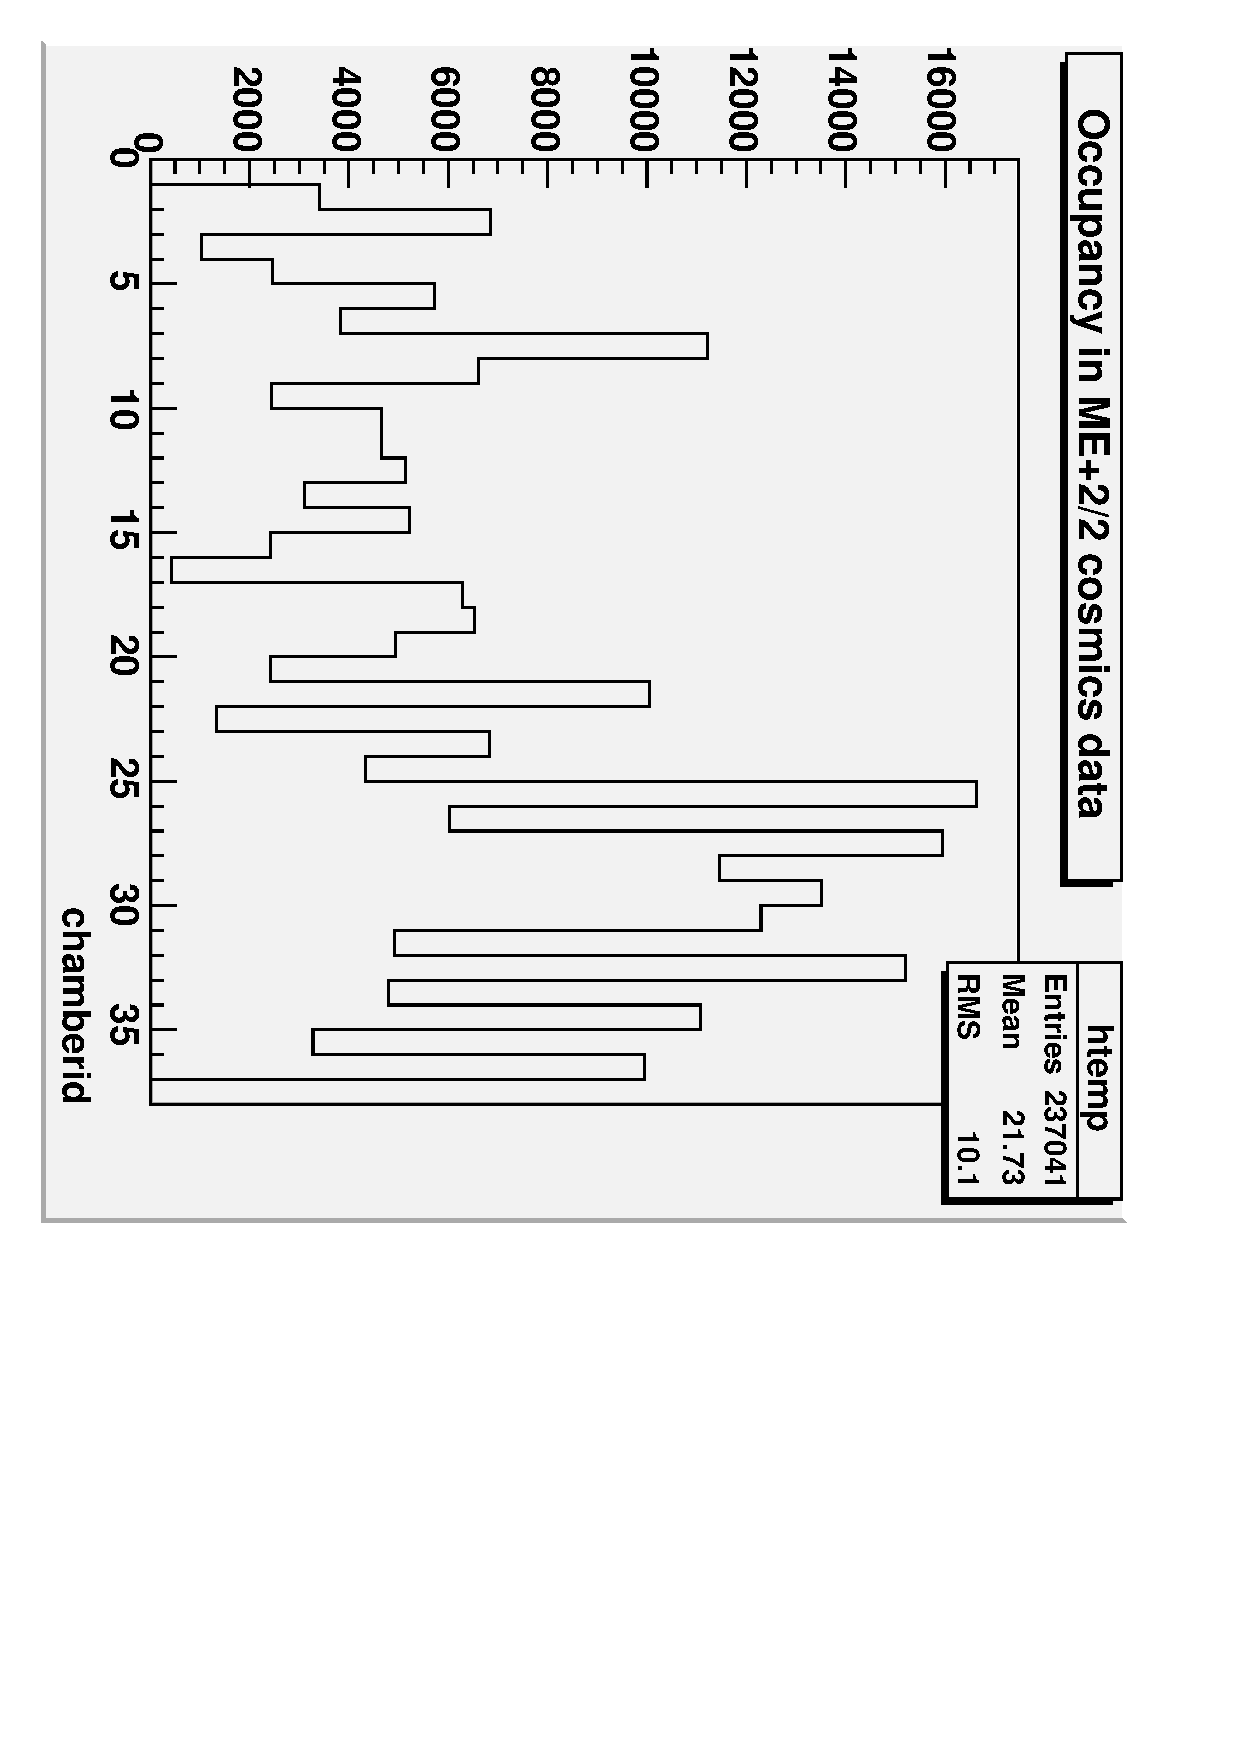
\includegraphics[height=\linewidth, angle=90]{data_occupancy_ME22.pdf}
\end{columns}
\end{frame}

\begin{frame}
\frametitle{What to do, what to do\ldots}
\small
\begin{itemize}
\item No sign of structure in cosmic ray residuals: they're just
  broad, as would be expected from granularity plus large uncertainty
  as to which wire group you're on
\item Maybe we can just call the cosmic ray case Gaussian and move on?
  (That is, interpret any failure to close as a {\it real} radial
  displacement of all chambers\ldots)
\item We'll need to specially handle granularity effects with
  beam-halo, but not yet
\item Inner ring (ME+2/1), being intermediate between ``large gaps''
  and ``nearly continuous,'' could be a difficult case
\item No need to modify the code now if we don't worry about
  granularity in cosmic rays
\item We should not use beam-halo MC as a predictor of cosmic ray data!
\item Running a one-step-at-a-time alignment from ME+2/2 chamber 34 in
  both directions to chamber 16 (which has the least statistics) to
  check closure in the simplest algorithm
\end{itemize}

\label{numpages}
\end{frame}

\end{document}
